\title          {Advanced Systems Lab}
\author         {Erik Jonsson (\textit{jerik}) and Michael Bang (\textit{mbang})}

\documentclass{article}
\usepackage[utf8]{inputenc}
\usepackage{amsmath}
\usepackage{amssymb}
\usepackage{float}
\usepackage{graphics}
\usepackage{changepage}
\usepackage{epstopdf}
\usepackage{graphicx}
    \DeclareGraphicsExtensions{.pdf,.png,.jpg,.eps}
    \graphicspath{{img/}}

\begin{document}
    \maketitle
    \tableofcontents

    \section{Implementation description}
        In our message passing system we have decided to make the client as simple as possible by placing as little logic as possible here. The middleware provides a well-defined API that the clients can use to interact with the messaging service. The middleware interacts with a database using SQL. Figure \ref{fig:implementation_high_level} is a graphical representation of our system. In the following we give an explanation of the life of a request, starting from and ending at the client. The reader can follow these steps on Figure \ref{fig:implementation_high_level}.
         \begin{figure}[H]
            \hspace{-2.8cm}
             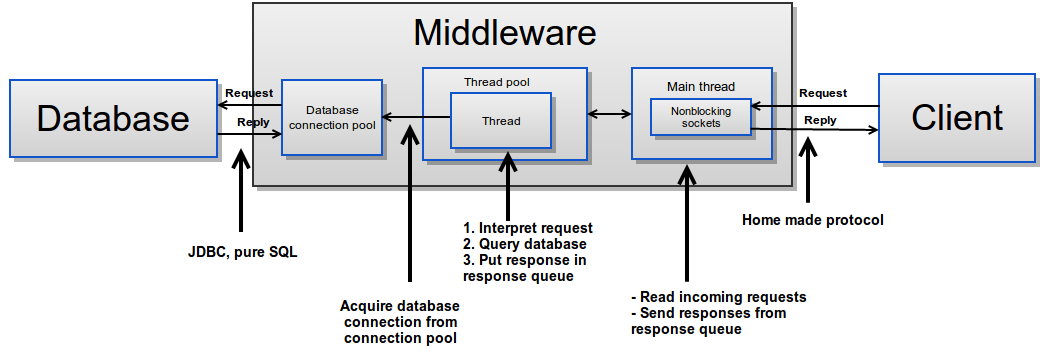
\includegraphics[scale=0.50]{implementation_high_level}
             \caption{Graphical representation of implementation}
             \label{fig:implementation_high_level}
         \end{figure}
         \begin{enumerate}
             \item Client X sends request to middleware
             \item Middleware receives request on non-blocking socket in the network i/o
             \item Middleware passes raw request data on to worker thread X from the worker thread-pool
             \item Worker thread Y interprets the request
             \item Worker thread Y fetches a database connection from the database connection-pool, and performs a query matching the client's request
             \item Depending on the result of the query, worker thread Y figures out what to respond to the client and puts the response in the response queue
             \item Next time the network i/o thread goes through the response queue, it will find response Y and send it to client X
         \end{enumerate}
         
         There can, of course, be more than one middleware in our system. In this case the figure would be the same, as seen from the viewpoint of a client, because each client is connected to exactly one middleware.\\
        In the following subsections we explain our design decisions with regard to each component of our system: client, middleware, and database.

        \subsection{Client}
            As noted earlier, we have tried to keep the implementation of our client as simple as possible. This means that our client implementation only consists of code that implements the API described in Appendix \ref{sec:message_protocol_api}. Basically, our client code is a library that can be used in other Java applications to communicate with our middleware.\\
            \\
            The client has the following important Java \textbf{packages} and \textit{classes}:
            \begin{itemize}
                \item \textbf{asl}
                    \begin{itemize}
                        \item \textit{ThorBangMQ} - 'API': implements sendMessage, popMessage etc.
                        \item \textit{Message} - Representation of a message
                    \end{itemize}
                \item \textbf{asl.network}
                \begin{itemize}
                     \item \textit{SocketTransport} - Transport layer using sockets
                 \end{itemize} 
                \item \textbf{asl.infrastructure}
                 \begin{itemize}
                    \item \textit{MemoryLogger} - Logs to memory with the possibility to dump logs to a file later
                \end{itemize}
                \item \textbf{asl.infrastructure.exceptions}
                \begin{itemize}
                    \item \textit{InvalidClientException} - Invalid client id
                    \item \textit{InvalidQueueException} - Invalid queue id
                    \item \textit{InvalidMessageException} - Invalid message id
                    \item \textit{ServerException} - Unknown exception at server, something is very wrong
                \end{itemize}
            \end{itemize}

        \subsection{Middleware}
            \label{sec:description_middleware}
            In our middleware we have chosen to use non-blocking sockets instead of blocking sockets since it as a few properties that we like, one of which is that we don't have to spawn a new thread for every client that connects. This means that it has a very small impact on our server when a client connects, and that we can support many more clients simultaneously since the amount of threads in our program doesn't have to be linear to the amount of clients currently connected. There is an obvious disadvantage to choosing non-blocking sockets over blocking sockets though, which is that it can be harder to think about, implement, and work with non-blocking sockets.\\
            \\
            In an attempt to make our implementation simpler we decided to perform all network i/o in one thread of our program. Since we want to be able to handle multiple requests simultaneously, we pass data from the network i/o-thread to worker threads for interpretation and handling. These worker threads interpret incoming data and perform the database queries needed to handle requests. Responses to these requests are put in a response queue, which the network i/o-thread will empty as often as it can, by sending sending replies directly to clients.\\
            \\
            By moving interpretation and handling of requests to a thread different from the network i/o-thread, we have a place to perform our (blocking) calls to the database without blocking incoming requests. This is not entirely true though, since if there are more simultaneous requests than there are worker threads, the network i/o thread will be blocked when trying to spawn a new worker thread, since there are no more worker threads available.\\
            \\
            We have chosen to use a thread-pool for our worker threads in order to avoid the overhead of creating and deleting threads all of the time, and at the same time bound the  number of worker threads our program will spawn. This should make our system able to handle many requests than we have threads, at the cost of slower response times. It is important to note that this also means that the amount of simultaneous requests that our implementation can handle is equal to the minimum of the number of worker threads and the number of database connections. This is the case since a worker thread always needs a database connection to do its work (unless it received a malformed request, which shouldn't happen during our tests).\\
            \\
            With regard to database connections, we have chosen to use a connection-pool to avoid the overhead of setting up a new connection to the database each time we want to perform a query.\\
            \\
            The middleware consists of the following important Java \textbf{packages} and \textit{classes}:
            \begin{itemize}
                \item \textbf{asl}
                \begin{itemize}
                    \item \textit{Main} - Entry point of the program
                    \item \textit{IntervalLogger} - Logs test data every x second, configurable
                    \item \textit{GlobalCounters} - Holds global counters used during tests
                    \item \textit{Message} - Representation of a message
                    \item \textit{ServerSettings} - Configurable parameters of the server
                \end{itemize}
                \item \textbf{asl.infrastructure}
                \begin{itemize}
                    \item \textit{MemoryLogger} - Logs to memory with the possibility to dump logs to a file later
                \end{itemize}
                \item \textbf{asl.infrastructure.exceptions}
                \begin{itemize}
                    \item \textit{InvalidClientException} - Invalid client id
                    \item \textit{InvalidQueueException} - Invalid queue id
                    \item \textit{InvalidMessageException} - Invalid message id
                    \item \textit{ServerException} - Unknown exception at server, something is very wrong
                \end{itemize}
                \item \textbf{asl.network}
                \begin{itemize}
                    \item \textit{SocketTransport} - Transport layer using sockets
                \end{itemize}
                \item \textbf{asl.persistence}
                \begin{itemize}
                    \item \textit{PostgresPersistence} - Use Postgres as storage
                    \item \textit{InMemoryPersistence} - Use local memory as storage
                    \item \textit{LyingPersistence} - Don't store anything
                \end{itemize}
            \end{itemize}
            ~\\
            It should be noted that in our implementation of \textit{Pop message} we are using 'Peek message'. This causes two accesses to the database whenever a client performs a \textit{Pop message}-request that returns a message. We only realized this after doing our tests, which is why we kept the implementation as described.

        \subsection{Database}
            We have chosen to use a simple database schema with three tables: messages, queues, and clients. This schema is illustrated on Figure \ref{fig:database_schema}. We have used the following two multicolumn-indexes on the \textit{messages}-table: \textit{(receiver\_id, queue\_id, time\_of\_arrival)} and \textit{(receiver\_id, queue\_id, priority)}. 
            \begin{figure}[H]
                \centering
                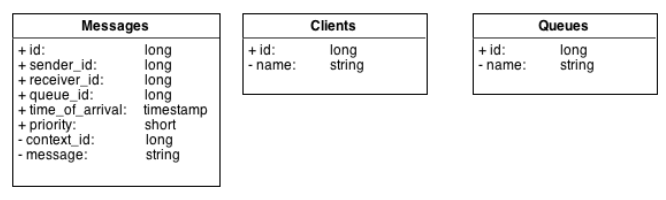
\includegraphics[scale=0.50]{database_schema}
                \caption{Database schema}
                \label{fig:database_schema}
            \end{figure}
            ~\\
            When clients send messages to multiple queues at once, we have chosen to replicate messages in queues rather than having a many-to-many relationship in the database. This decision could affect performance since we're inserting more messages than we would, had we chosen to use a many-to-many relationship.\\
            \\
            Communication between the middleware and our database is done using JDBC, and we make SQL queries directly from our Java code. We decided not to use stored procedures, even though it requires slightly less data to represent each query, because we found it easier to implement and debug SQL directly in our Java code.\\
            \\
            TODO: Write something about how our tests have been done without any indexes.

        \subsection{Communication protocol and API}
            We have chosen to use a very simple messaging protocol between the clients and the middleware. It uses an end of message token to differentiate messages from each other as we found it simpler to implement, compared to defining packets with headers containing message length and so on. We decided that our end of message token should be null, i.e. "\textbackslash0". All messages should be encoded in UTF8.\\
            Interpretation of requests and responses using our protocol is implemented in both server and client, in the SocketTransport classes. The full description of the communication protocol and API can be found in Appendix \ref{sec:message_protocol_api}.

    \section{Testing infrastructure}
        Our testing infrastructure is written in Python and does the following:
        \begin{itemize}
            \item Starts and stops servers
            \item Starts and stops experiments
            \item Fetches logs
            \item Generates graphs
        \end{itemize}
        ~\\
        Figure \ref{fig:testing_infrastructure} gives a graphical interpretation of our testing infrastructure.\\
         \begin{figure}[H]
             \centering
             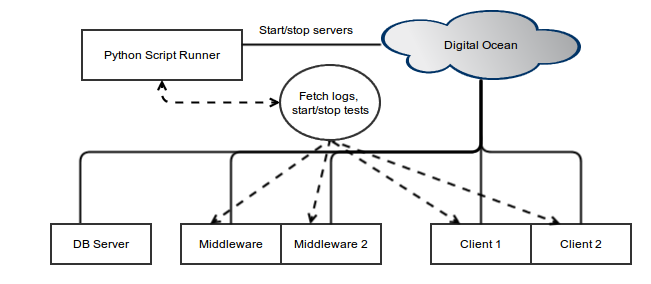
\includegraphics[scale=0.50]{testing_infrastructure}
             \caption{Graphical representation of our testing infrastructure}
             \label{fig:testing_infrastructure}
         \end{figure}
        The infrastructure consists of 4 files:
        \begin{description}
            \item[main.py] Interface to start tests, see servers currently running etc.
            \item[infrastructure.py] Functions doing the actual infrastructure work.
            \item[droplets.py] Functions to start and stop servers (specific to DigitalOcean cloud provider).
            \item[gnuplot.py] Plots data.
        \end{description}
        ~\\
        Tests are defined by creating a folder in the test-definitions directory and creating three files: \textit{conf.txt}, which defines the configuration of a server, \textit{test.txt}, which defines the configuration of the clients and the number of servers and clients the test should be deployed on, and \textit{gnuplot.sh} which generates gnuplots when called with a test-result file as an argument.\\
        \\
        Other than the files described above, our testing infrastructure relies on the following python libraries: 
        \begin{description}
            \item[python-digitalocean] which can be installed via pip or found at \textit{https://pypi.python.org/pypi/python-digitalocean}.
            \item[psycopg2] which can be found at \textit{https://pypi.python.org/pypi/psycopg2}.
        \end{description}
        ~\\
        It should be noted that our testing infrastructure is very simple in that, for instance, it doesn't check for errors while running; it just assumes that everything executes successfully and continues on, even though that is not the case. We found this to be a somewhat of a mistake since it has caused us quite a bit of trouble during our testing.

    \section{Test definitions}
        \label{sec:test_definitions}
        This section contains a description of the tests that we performed during our measurements of our system. These tests can be configured in various ways in order to test different parts of our system. For all tests where nothing else is mentioned, the amount of messages in the database has been kept steady at around 20,000 messages, and the size of messages is very low (around 5 bytes).

        \subsection{Send and Pop Same Client}
            In this test all client threads continuously send 'SendMessage' and 'PopMessage' requests to the server (described in Appendix \ref{sec:message_protocol_api}). Each client thread sends a message to itself, then pops the message it just sent, and then repeats. This test is designed to keep the amount of messages in the database stable, while potentially putting a lot of load on the database - depending on the configuration of the parameters. The test is configurable in: the number of (identical) threads to be spawned, time the test should run, the size of messages sent, the number of queues being used, and the amount of time each thread should sleep between sending requests. In all tests where nothing else is mentioned, the waiting time between requests is 0.\\
            \\
            \\
            Tests of this type perform the same amount of 'SendMessage' and 'PopMessage' requests, which means that the amount of messages in the system is kept stable. We expect that this test could put a lot of load on the server, especially if the amount of sleep-time is very low.

        \subsection{Standard test}
            \label{sec:standard_test}
            This test is an implementation of the test described in the project description, which we're supposed to be using for the traces. Our interpretation of the description, and our implementation, is as follows: A number of one-way clients bounce a single message randomly between each other, incrementing a counter in the message. Each one-way client keeps performing \textit{Pop message}-requests, checking if he got the message. A number of two-way clients each have a partner assigned, with whom they keep sending messages back and forth. Each two-way client keeps sending \textit{Pop message}-requests until he receives a message from his partner, and then sends a reply back. From this description we should note that the amount of \textit{Send Message}-requests doesn't change when incrementing the number of one-way clients increases, but it does when the number of two-way clients increases. Also to be noted, the number of \textit{Pop message}-requests increases when incrementing either of the two types of clients.\\
            \\
            The test is configurable in the amount of one-way clients and two-way clients it should use. Only too late did we realize that it would have been nice to be able to configure the size of messages sent, and the number of queues the messages are distributed over.\\
            \\
            Tests of this type perform many more 'PopMessage' requests than 'SendMessage' requests, but most of these 'PopMessage' requests will not actually find a message to pop, causing the total number of messages in the system to be kept stable.

        \subsection{Push peek pop}
            In this test a single client performs a configurable amount of a single type of request. This test is used for micro benchmarking each type of request.
            The test can be configured in: the type of requests sent and the amount of requests sent. This test can't be configured from the command line, and must be performed manually.\\
            \\
            Depending on the request being benchmarked, the amount of messages will differ. \textit{Send Message} requests, for instance, will increase the amount of messages in the system, while \textit{Pop message} will decrease the amount of messages in the system.

        \subsection{Timing measurements on the middleware}
            On the middleware we perform some timing measurements, measuring how much time is spent in different parts of our system. These names that we use for these parts are:\\
            \\
            \indent \textbf{IPersistence} which uses JDBC to query our database. Time spent in this class includes: think time for a database query and network delays from our middleware to the database and back again.\\
            \\
            \indent \textbf{Client Request Worker} which interprets user requests. Time spent in this class includes: string manipulation to interpret user requests, calling of methods in IPersistence, creating a response for the client and putting it in the response queue. The time spent in IPersistence is subtracted from the time measured in this class such that time measured for this class doesn't include the time it takes to perform calls in IPersistence.\\
            \\
            \indent \textbf{Socket I/O \& Queuing} which handles communication with clients. Time spent in this class includes: reading from and writing to a client socket, handing data read from client sockets to a worker thread, and the time requests spend waiting to get handed to a worker thread.
            \\
            \\
            Figure \ref{fig:timing_measurements} is a graphical representation of these measurements.\\
            \begin{figure}[H]
                \centering
                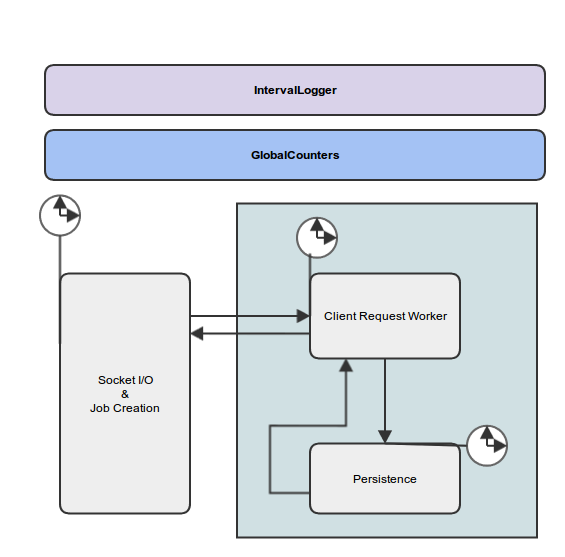
\includegraphics[scale=0.50]{timing_measurements}
                \caption{Graphical representation of timing measurements done on middleware}
                \label{fig:timing_measurements}
            \end{figure}

    \section{Tests and results}
        \label{sec:tests_and_results}
        In this section we describe the tests we have performed, present the results and give a short commentary on what can be seen on the graphs. We interpret and analyze these results in Section \ref{sec:analysis}.\\
        \\
        In our tests we have focused on peeking, popping, and sending messages. We decided to have this focus because we work under the assumption that these types of requests are vastly more frequent than all other types of requests (create queue, remove queue etc.), and that the performance of the system as a whole will be dominated by these three types of requests.\\
        \\
        We have performed our tests using machines from the cloud hosting provider DigitalOcean.com, from whom we got a 200\$ coupon to run experiments. Running our tests on a cloud host has some obvious downsides w.r.t. the results of our tests, since we can't know for sure which hardware our tests are run on, and if we are sharing this hardware with anyone.\\
        We have run all of our experiments on machines with: 4GB memory, SSD storage, and 2 logical CPU cores. Due to the way DigitalOcean provide their servers, we can't really tell how much computing power these logical CPUs provide, or whether there are any neighbors on the hardware. In order to compensate for this we've run all of our experiments for at least 10 minutes each, to see whether the observed performance is somewhat consistent.\\
        \\
        It is important to note that all of the following tests use blocking sockets (on the client side) to send requests. This means that each of our clients can not have more than one request simultaneously. In the literature this is referred to as a closed system.\\
        \\
        In order to try to explain the performance of our system, we have identified the following parameters that we wish to test.
        \begin{itemize}
            \item Client
            \begin{itemize}
                \item Client threads per client machine
            \end{itemize}
            \item Middleware
            \begin{itemize}
                \item Size of messages
                \item Total number of clients
                \item Frequency of requests
                \item Number of middleware instances
                \item Number of database connections
                \item Number of worker threads
                \item Impact of using database vs. not storing messages at all
            \end{itemize}
            \item Database
            \begin{itemize}
                \item Size of dataset
                \item Number of queues which messages are distributed over
            \end{itemize}
        \end{itemize}

        \subsection{Code profiling}
            In order to figure out exactly where our code spends the most time, we've used the code profiling tool VisualVM (\textit{http://visualvm.java.net/}). We have performed code profiling during multiple different tests with multiple different configurations. Every time we ran the profiler we got almost identical results. The profiling runs shown on Figure \ref{fig:code_profiling_send_pop_same_client} and \ref{fig:code_profiling_standard_test} were run for approx. 3 minutes with 80 clients sending very small messages (around 5 bytes). These two tests show the general results we got with all configurations of these two types of tests. Our code spends almost all of the time, as shown on Figure \ref{fig:code_profiling_send_pop_same_client} and \ref{fig:code_profiling_standard_test}, communicating with and waiting for the database. In fact, the top 3 most time consuming tasks are all due to communication with the database. If we put the time consumption of these tasks together, they add up to 83.1\% for 'Send and Pop Same Client' and 87.5\% for 'standard test'.
            \begin{figure}[H]
                \hspace{-1.5cm}
                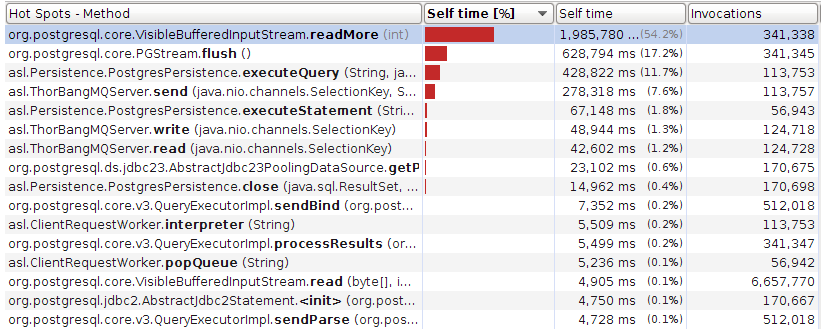
\includegraphics[scale=0.50]{code_profiling_send_pop_same_client}
                \caption{3 minutes of profiling during 'Send and Pop Same Client' with 80 clients, very small messages}
                \label{fig:code_profiling_send_pop_same_client}
            \end{figure}
            \begin{figure}[H]
                \hspace{-1.5cm}
                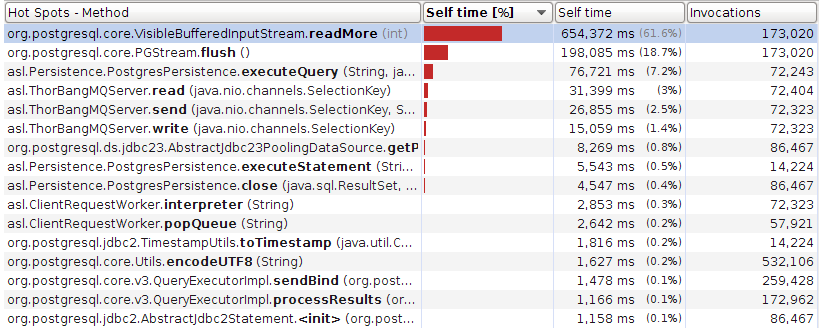
\includegraphics[scale=0.50]{code_profiling_standard_test}
                \caption{3 minutes of profiling during 'Standard test' with 80 clients, very small messages}
                \label{fig:code_profiling_standard_test}
            \end{figure}
            ~\\
            On both Figures we also see that \textit{ThorBangMQServer.read} and \textit{ThorBangMQServer.send} take up a lot of time: 8.8\% for 'Send and Pop Same Client' and 5.5\% for 'Standard test'. These two calls are responsible for communication with clients, where 'read' gets clients' requests and 'send' sends replies to clients.\\
            \\
            The last thing we note is that 'ThorBangMQServer.write' takes up 1.3\% and 1.4\% of 'Send and Pop Same Client' and 'Standard test' respectively. This method is responsible for putting responses into the response queue (as explained in Section \ref{sec:description_middleware}) and is performed by worker threads when they are done handling a client's request.

            % Bottlenecks
            % Most expensive operations that determine the overall performance

        \subsection{Long traces}
            The figures in this section show the overall stability of the system while under moderate to high system load for 2 hours or more. Each of the following tests are of the type \textit{Standard test} and have been run with different parameters, increasing the number of database connections and worker threads, and the number of clients. In these tests we expect to see that the system behaves in a somewhat stable manner (at least for lower numbers of clients) meaning that we have a low standard deviation of our measurements. We expect that the throughput will go up as the number of clients and worker-threads and database connections increases since, as described in Section \ref{sec:description_middleware}, the number of database connections and worker-threads bounds the amount of requests that will be handled simultaneously by our middleware. We don't think that this will scaling though, since increasing the number of database connections gives the opportunity to put more load on the database which, at some point, will not be able to cope with the increased load.\\
            \\
            All of the following graphs have been plotted with the throughput of reads and writes individually, and all have many more reads than writes for the reasons described in Section \ref{sec:standard_test}.\\

            \begin{figure}[H]
                \hspace{-1.5cm}
                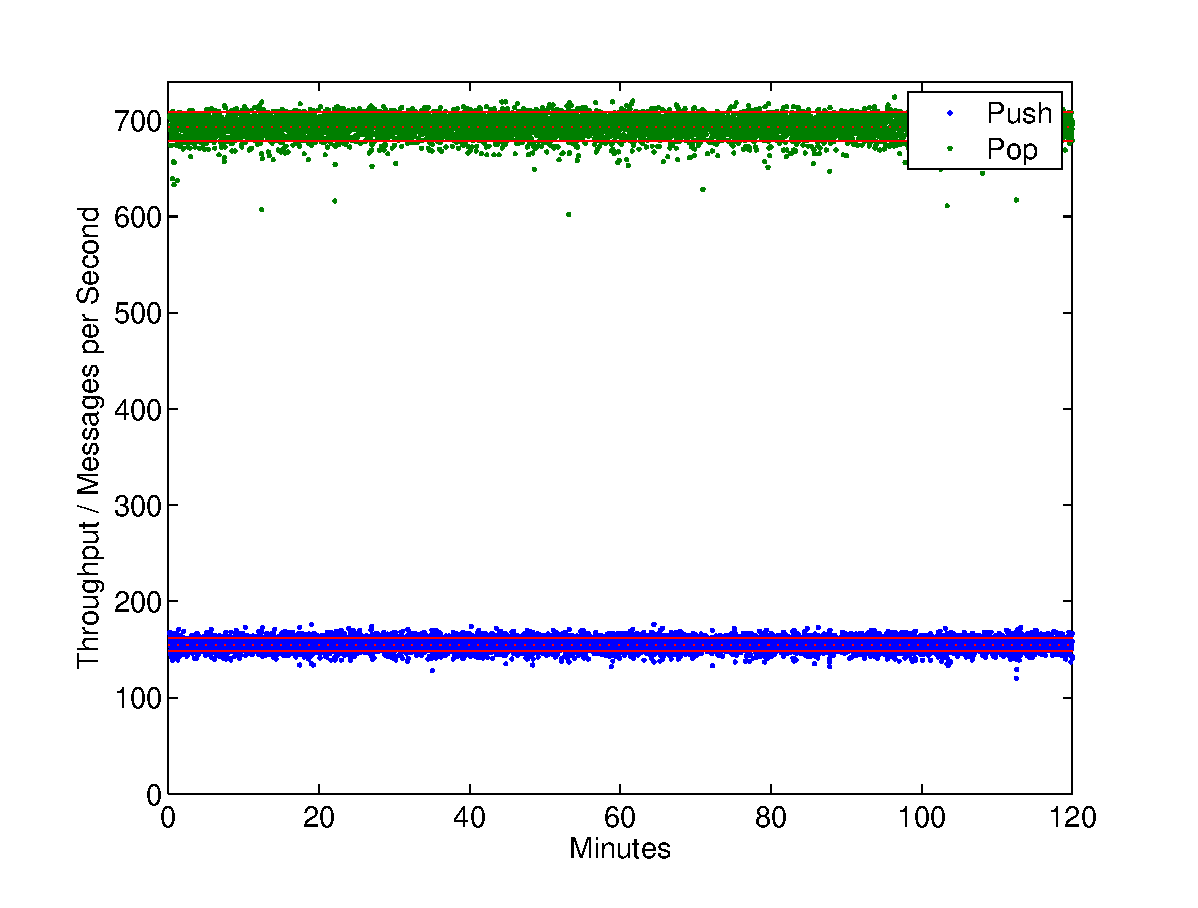
\includegraphics[scale=0.750]{2h_100threads_standardTest_100_50}
                \caption{The throughput of the system while under load from the \textit{Standard Test} with 100 one-way clients and 50 two-way clients. Using 1 middleware with 100 worker threads and 100 database connections. The dotted red line shows the average throughput and the solid lines the standard deviation.}
                \label{fig:2h_100threads_standardTest_100_50}
            \end{figure}
            ~\\
            \\
            On Figure \ref{fig:2h_100threads_standardTest_100_50}, where we have a total of 150 clients, using 100 worker threads and database connections in the middleware, we see that the throughput of both \textit{Pop message} and \textit{Send message} stays very stable throughout the whole test, showing [TODO] \textit{Pop message} and [TODO] \textit{Send message} per second, with a standard deviation of [TODO] and [TODO] respectively.\\
            \\
            On Figure \ref{fig:2h_30threads_standardTest_500_250}, where we have decreased the number of worker threads and database connections to 30 but increased the number of total clients to 750, we see that the throughput has gone up. This is especially the case for \textit{Pop message} requests, where we also see that standard deviation has increased significantly.
            \begin{figure}[H]
                \hspace{-1.5cm}
                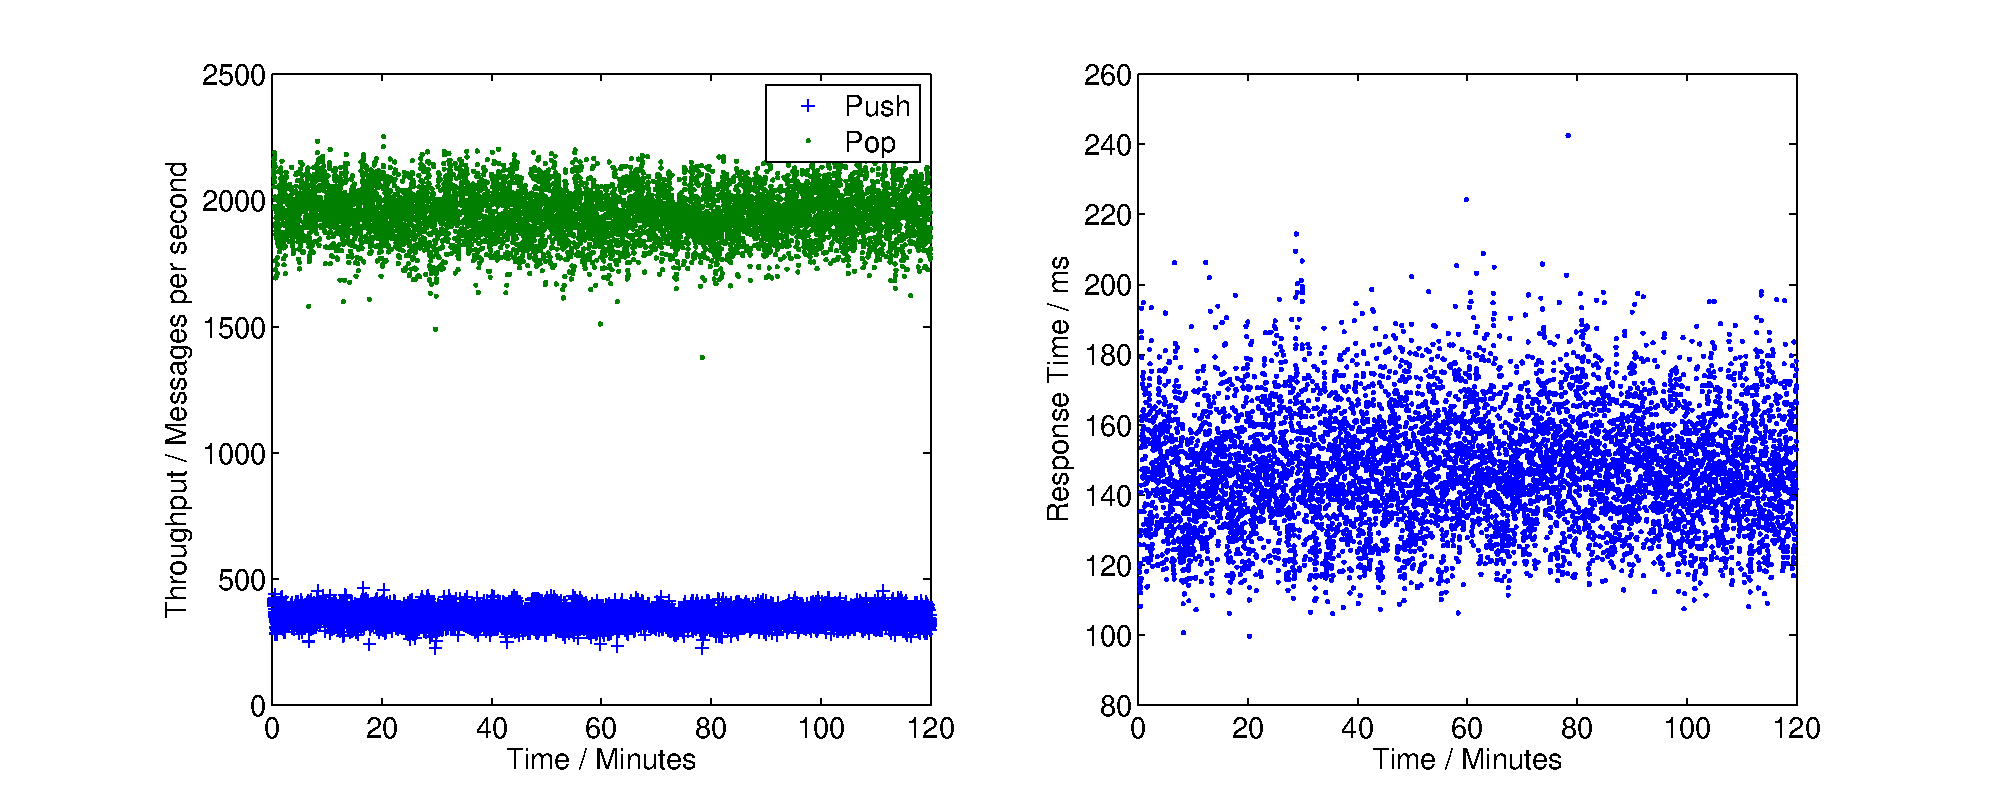
\includegraphics[scale=0.750]{2h_30threads_standardTest_500_250}
                \caption{The throughput of the system while under load from the \textit{Standard Test} with 500 one-way clients and 250 two-way clients. Using 1 middleware with 30 worker threads and 30 database connections. The dotted red line shows the average throughput and the solid lines the standard deviation.}
                \label{fig:2h_30threads_standardTest_500_250}
            \end{figure}
            ~\\
            \\
            On Figure \ref{fig:2h_100threads_standardTest_500_250} we have increased the number of worker threads and database connections to 100, but kept the number of clients at 750. Here we see that the throughput total throughput of requests hasn't increased very much, but that the standard deviation of especially \textit{Pop message} requests has increased.
                
            \begin{figure}[H]
                \hspace{-1.5cm}
                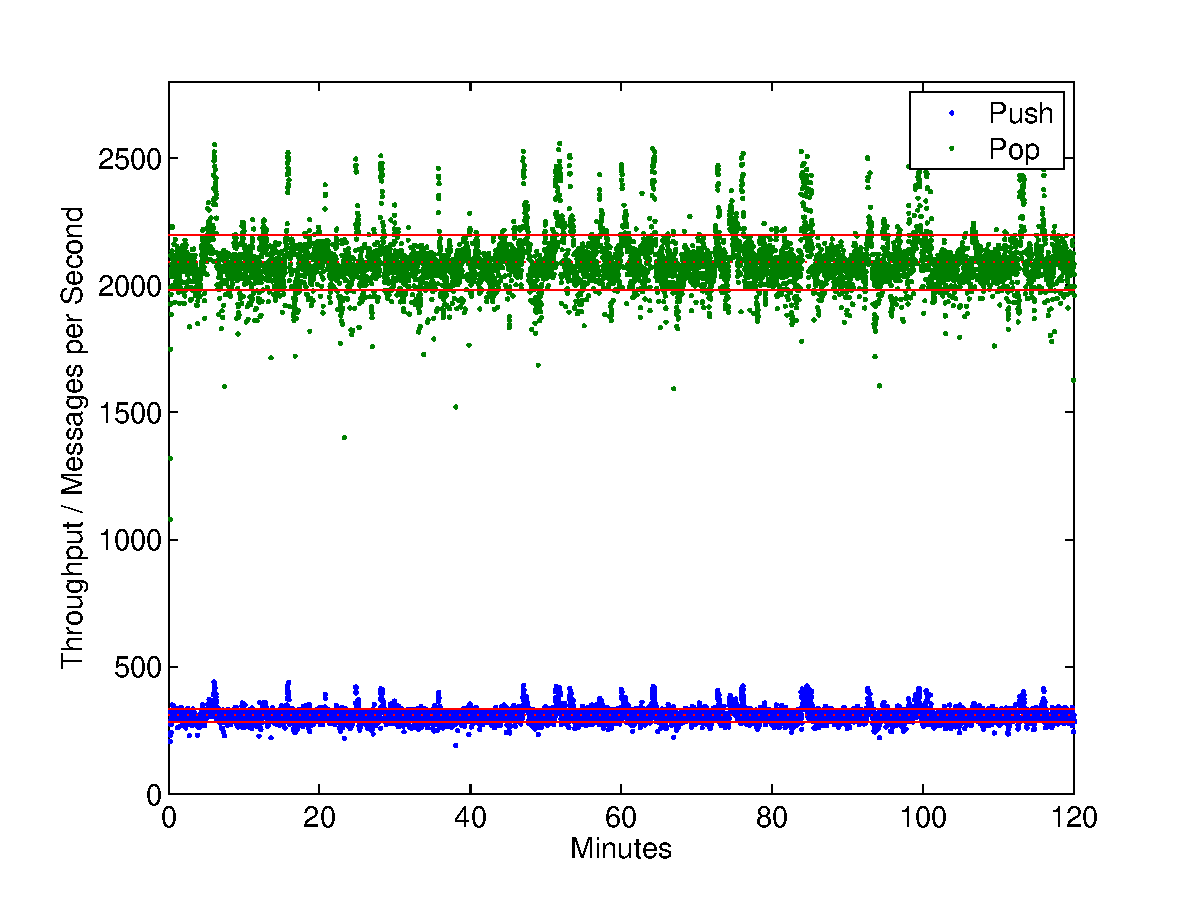
\includegraphics[scale=0.750]{2h_100threads_standardTest_500_250}
                \caption{The throughput of the system while under load from the \textit{Standard Test} with 500 one-way clients and 250 two-way clients. Using 1 middleware with 100 worker threads and 100 database connections. The dotted red line shows the average throughput and the solid lines the standard deviation.}
                \label{fig:2h_100threads_standardTest_500_250}
            \end{figure}
            ~\\
            \\
            On the longest running trace we have, running a total of 4 hours, we had a total of 300 clients and 30 worker threads and database connections in the middleware. The results of this test is shown on Figure \ref{fig:4h_throughput}. Here we see that the system behaves in a very stable manner throughout the  test.

            \begin{figure}[H]
                \hspace{-4.5cm}
                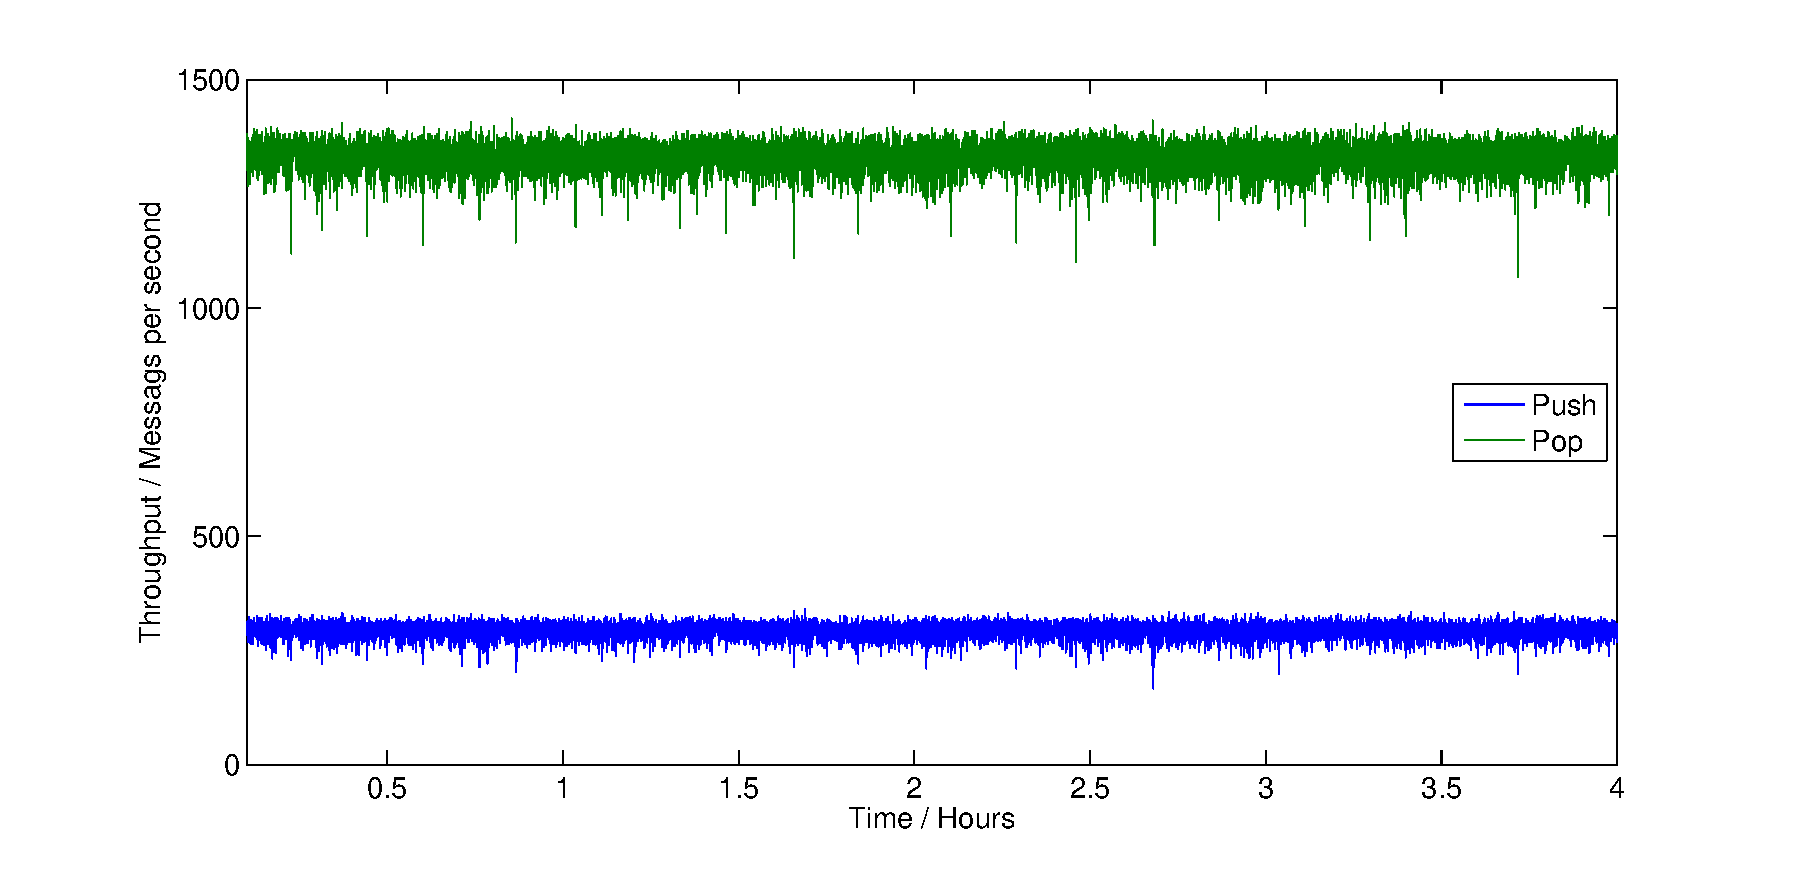
\includegraphics[scale=0.750]{4h_throughput}
                \caption{The throughput of the system while under load from the \textit{Standard Test} with 200 one-way clients and 100 two-way clients. Using 1 middleware with 30 worker threads and 30 database connections. The dotted red line shows the average throughput and the solid lines the standard deviation.}
                \label{fig:4h_throughput}
            \end{figure}
            ~\\
            ~\\
            Table \ref{table:long_trace_test_summary_sendmessage} and \ref{table:long_trace_test_summary_popmessage} give a summary of the results of our long traces. In these summaries we see that the standard deviation of both types of requests increases as the number of clients increases. We also see that the throughput goes up as the number of clients increases.

            \begin{table}[H]
                \caption{Summary of results of Send Message from long traces}
                \label{table:long_trace_test_summary_sendmessage}
                \begin{adjustwidth}{-2cm}{}
                    \begin{tabular}{|c|c|c|c|c|}
                        \hline 
                        \textbf{1-way} & \textbf{2-way} & \textbf{Threads/DB-conns} & \textbf{Throughput Send Message (msgs/s)} & \textbf{Standard Deviation}\\ 
                        \hline 
                        500 & 250 & 100/100 &309.22 &26.45\\
                        \hline
                        100 & 50 & 100/100 &155.13 &6.6\\
                        \hline 
                        500 & 250 & 30/30 &350.89 &29.85\\
                        \hline
                        200 & 100 & 30/30 &292.69 &24.33\\
                        \hline
                    \end{tabular} 
                \end{adjustwidth}
            \end{table}

            \begin{table}[H]
                \caption{Summary of results of Pop Message from long traces}
                \label{table:long_trace_test_summary_popmessage}
                \begin{adjustwidth}{-2cm}{}
                    \begin{tabular}{|c|c|c|c|c|}
                        \hline 
                        \textbf{1-way} & \textbf{2-way} & \textbf{Threads/DB-conns} & \textbf{Throughput Pop Message (msgs/s)} & \textbf{Standard Deviation} \\ 
                        \hline 
                        500 & 250 & 100/100 &2090.5 &108.25\\
                        \hline
                        100 & 50 & 100/100 &693.4 &15.33\\
                        \hline 
                        500 & 250 & 30/30 &1945.52 &101.31\\
                        \hline
                        200 & 100 & 30/30 &1326.23 &90.21\\
                        \hline
                    \end{tabular} 
                \end{adjustwidth}
            \end{table}

        \subsection{Micro benchmarks}
            The tests in this section are made to test the performance of single types of requests. The following tests have been performed on a single middleware with 50 worker threads and 50 database connections. The amount of worker threads and database connections should not matter to this test though, since we use only a single client which will only send the next request when it has received a reply to the previous (closed system). This is tested in Section \ref{sec:difference_in_dbcons_and_worker_threads}.

            \subsubsection{Send message}
                In this test a single client continuously sends \textit{send message} requests to the server. This means that the size of the dataset increases from 20,000 to 520,000 in the span of the test.\\
                \\
                On Figure \ref{fig:thinktime_500k_push} we see that the amount of time spent on each request is dominated by requests to the database, shown by the scattered dots in the top of the graph. In Table \ref{table:thinktime_500k_push} the data for this graph is given, showing that the time spent in IPersistence is at least an order of magnitude higher than the rest of the system. We also see that the standard deviation of time spent in IPersistence is much higher than it is for the two other measurements.\\
                Figure \ref{fig:responsetime_500k_push} shows the response time throughout the 500,000 \textit{Send message} requests. On this graph we see that the response time is rather stable, except for the scattered points in the top of the graph.

                \begin{figure}[H]
                    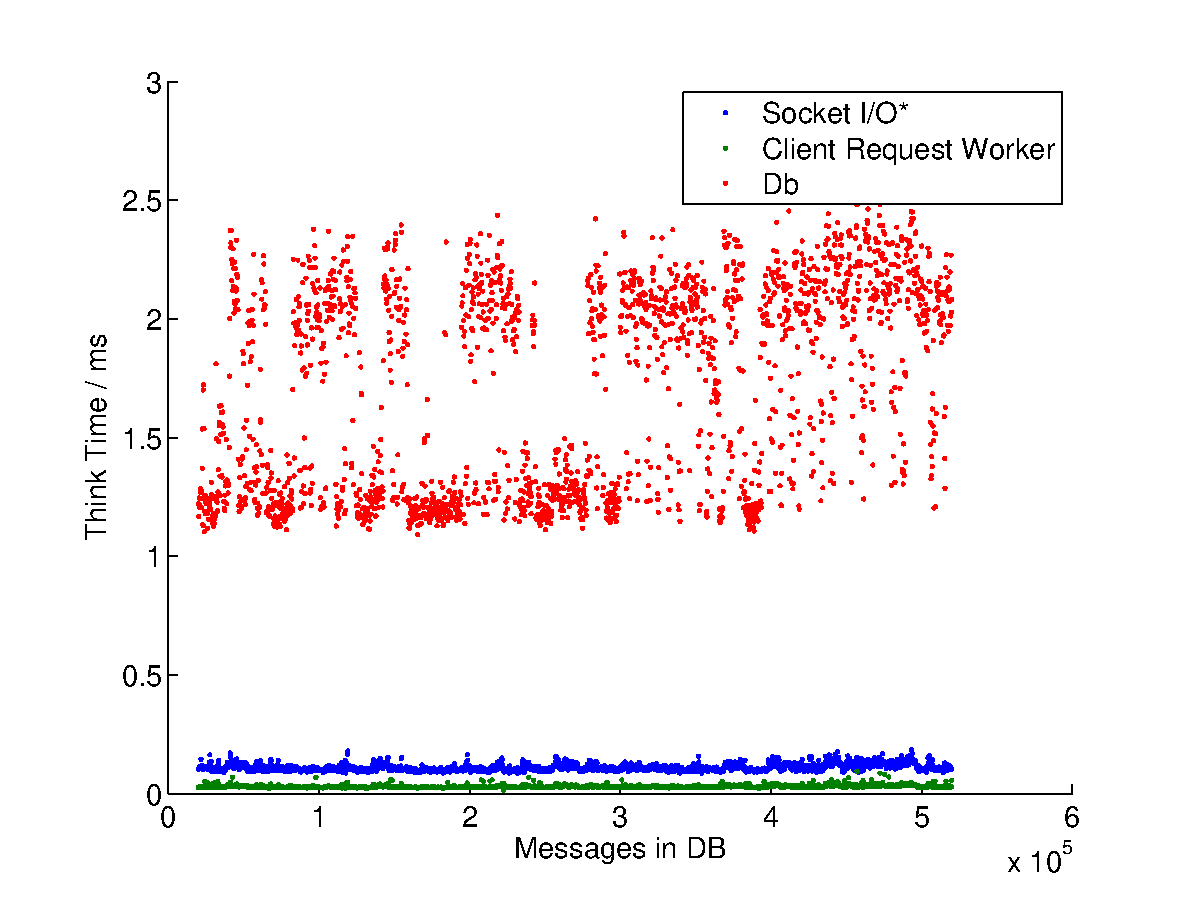
\includegraphics[scale=0.50]{thinktime_500k_push}
                    \caption{The think time for send message request. Each data point represents an individual request. A total of 500,000 requests sent sequentially each after the other.}
                    \label{fig:thinktime_500k_push}
                \end{figure}
                \begin{table}[H]
                    \begin{tabular}{|c|c|c|}
                        \hline 
                        \textbf{Component} & \textbf{Average Think Time} (ms) & \textbf{Standard Deviation (ms)} \\ 
                        \hline 
                        Socket I/O \& Queuing & $0.111 \pm 0.021$ &0.0145\\ 
                        \hline 
                        CRW & $0.0310 \pm0.099$ &0.0057\\ 
                        \hline 
                        IPersistence & $1.714 \pm 0.590$ &0.427\\ 
                        \hline 
                    \end{tabular}
                    \caption{Average think time, confidence interval, and standard deviation for 500,000 \textit{Send message} requests}
                    \label{table:thinktime_500k_push}
                \end{table} 
                
                \begin{figure}[H]
                    \includegraphics[scale=0.50]{responsetime_500k_push}
                    \caption{The response time for send message request. Each data point represents an individual request. A total of 500,000 requests sent sequentially each after the other.}
                    \label{fig:responsetime_500k_push}
                \end{figure}
                ~\\
                \\
                The raw data from this test can be found in the log-folder, in the subfolders
                \begin{itemize}
                    \item folders
                \end{itemize}

            \subsubsection{Pop message}
                In this test a single client continuously sends a total of 500,000 \textit{Pop message} requests. This test was run after the \textit{Send message} test described in the last subsection, which means that there was a total of 520,000 messages in the database when this test was started. In this test the amount of messages in the database goes from 520,000 to 20,000.\\
                \\
                On Figure \ref{fig:thinktime_500k_pop} we see that the think time has a very specific pattern over time. It seems that 


                \begin{figure}[H]
                    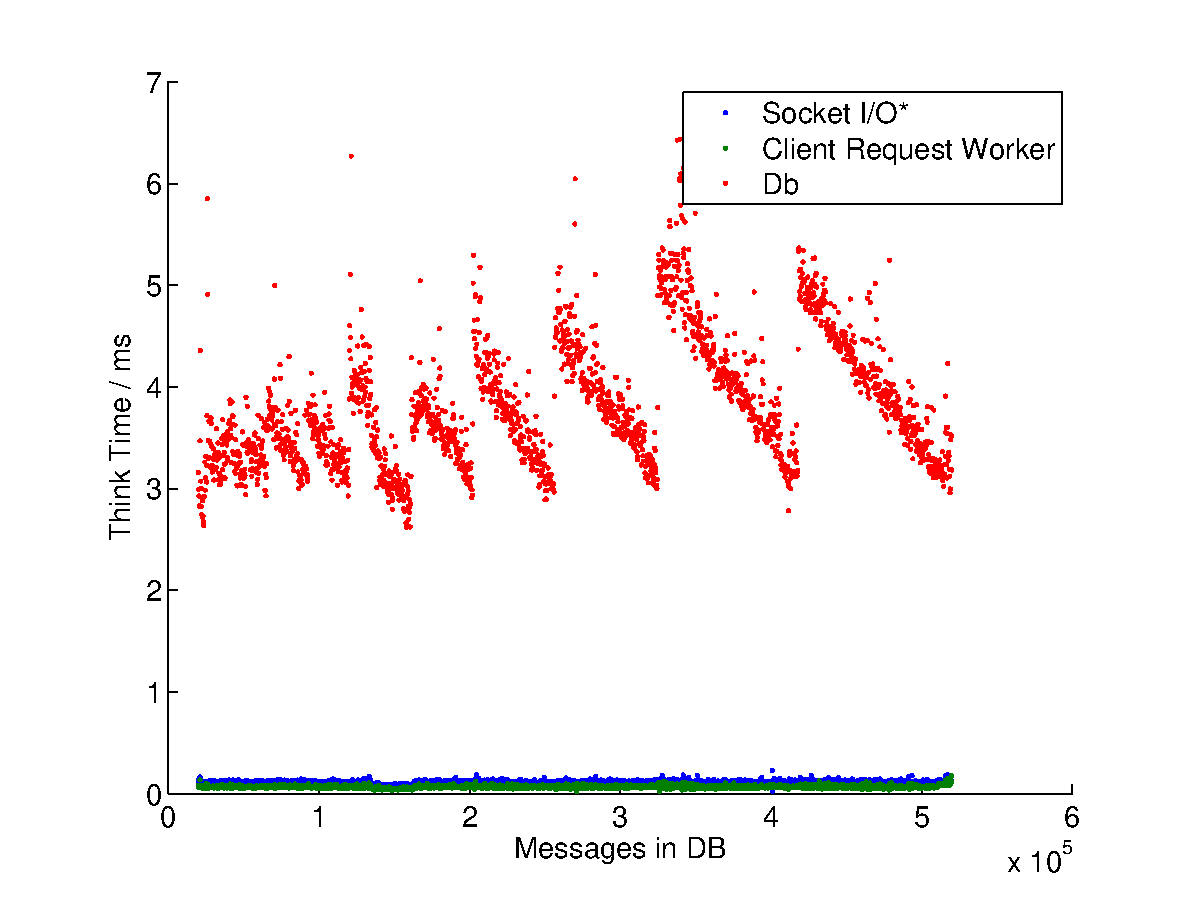
\includegraphics[scale=0.50]{thinktime_500k_pop}
                    \caption{The think time in the server for \textit{pop message} request. Each data point represents an individual request. A total of 500,000 requests.}
                    \label{fig:thinktime_500k_pop}
                \end{figure}

                \begin{table}[H]
                    \begin{tabular}{|c|c|c|}
                        \hline 
                        \textbf{Component} & \textbf{Average Think Time} (ms)  & \textbf{Standard Deviation (ms)} \\ 
                        \hline 
                        Socket I/O \& Queuing & $0.118\pm0.021$ &0.014 \\ 
                        \hline 
                        CRW & $0.069\pm0.023$ &0.013 \\ 
                        \hline 
                        IPersistence & $3.810\pm1.164$ &0.609 \\ 
                        \hline 
                    \end{tabular}
                \end{table}
                
                \begin{figure}[H]
                    \includegraphics[scale=0.50]{responsetime_500k_pop}
                    \caption{The response time for \textit{pop message} request. Each data point represents an individual request. A total of 500,000 requests sent sequentially each after the other.}
                    \label{fig:responsetime_500k_pop}
                \end{figure}                
                ~\\
                \\
                The raw data from these tests can be found in the log-folder, in the subfolders
                \begin{itemize}
                    \item folders
                \end{itemize}               
                
            \subsubsection{Peek message}
                \begin{figure}[H]
                    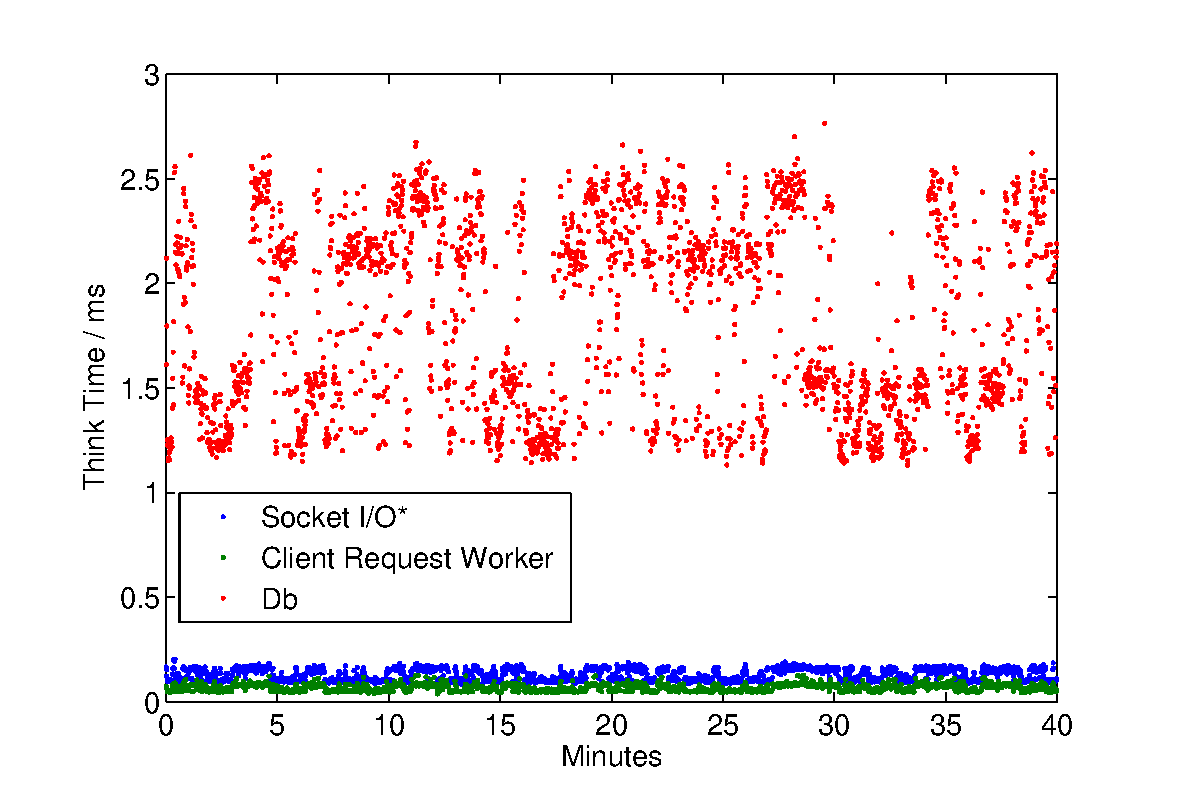
\includegraphics[scale=0.50]{thinktime_500k_peek}
                    \caption{The think time in the server for \textit{peek message} request. Each data point represents an individual request. A total of 500,000 requests sent sequentially each after the other.}
                    \label{fig:thinktime_500k_peek}
                \end{figure}
                \begin{table}[H]
                    \begin{tabular}{|c|c|c|}
                        \hline 
                        \textbf{Component} & \textbf{Average Think Time} (ms)  & \textbf{Standard Deviation (ms)} \\ 
                        \hline 
                        Socket I/O \& Queuing &$0.129\pm0.038$ &0.027\\ 
                        \hline 
                        CRW &$0.066\pm0.022$ &0.016\\ 
                        \hline 
                        IPersistence &$1.826\pm0.653$ &0.452\\ 
                        \hline 
                    \end{tabular}
                \end{table} 

                \begin{figure}[H]
                    \includegraphics[scale=0.50]{responsetime_500k_peek}
                    \caption{The response time for send message request. Each data point represents an individual request. A total of 500,000 requests sent sequentially each after the other.}
                    \label{fig:responsetime_500k_peek}
                \end{figure}
                ~\\
                \\
                The raw data from these tests can be found in the log-folder, in the subfolders
                \begin{itemize}
                    \item folders
                \end{itemize}

        \subsection{Difference in message size}
            \begin{figure}[H]
                    \hspace{-1.5cm}
                    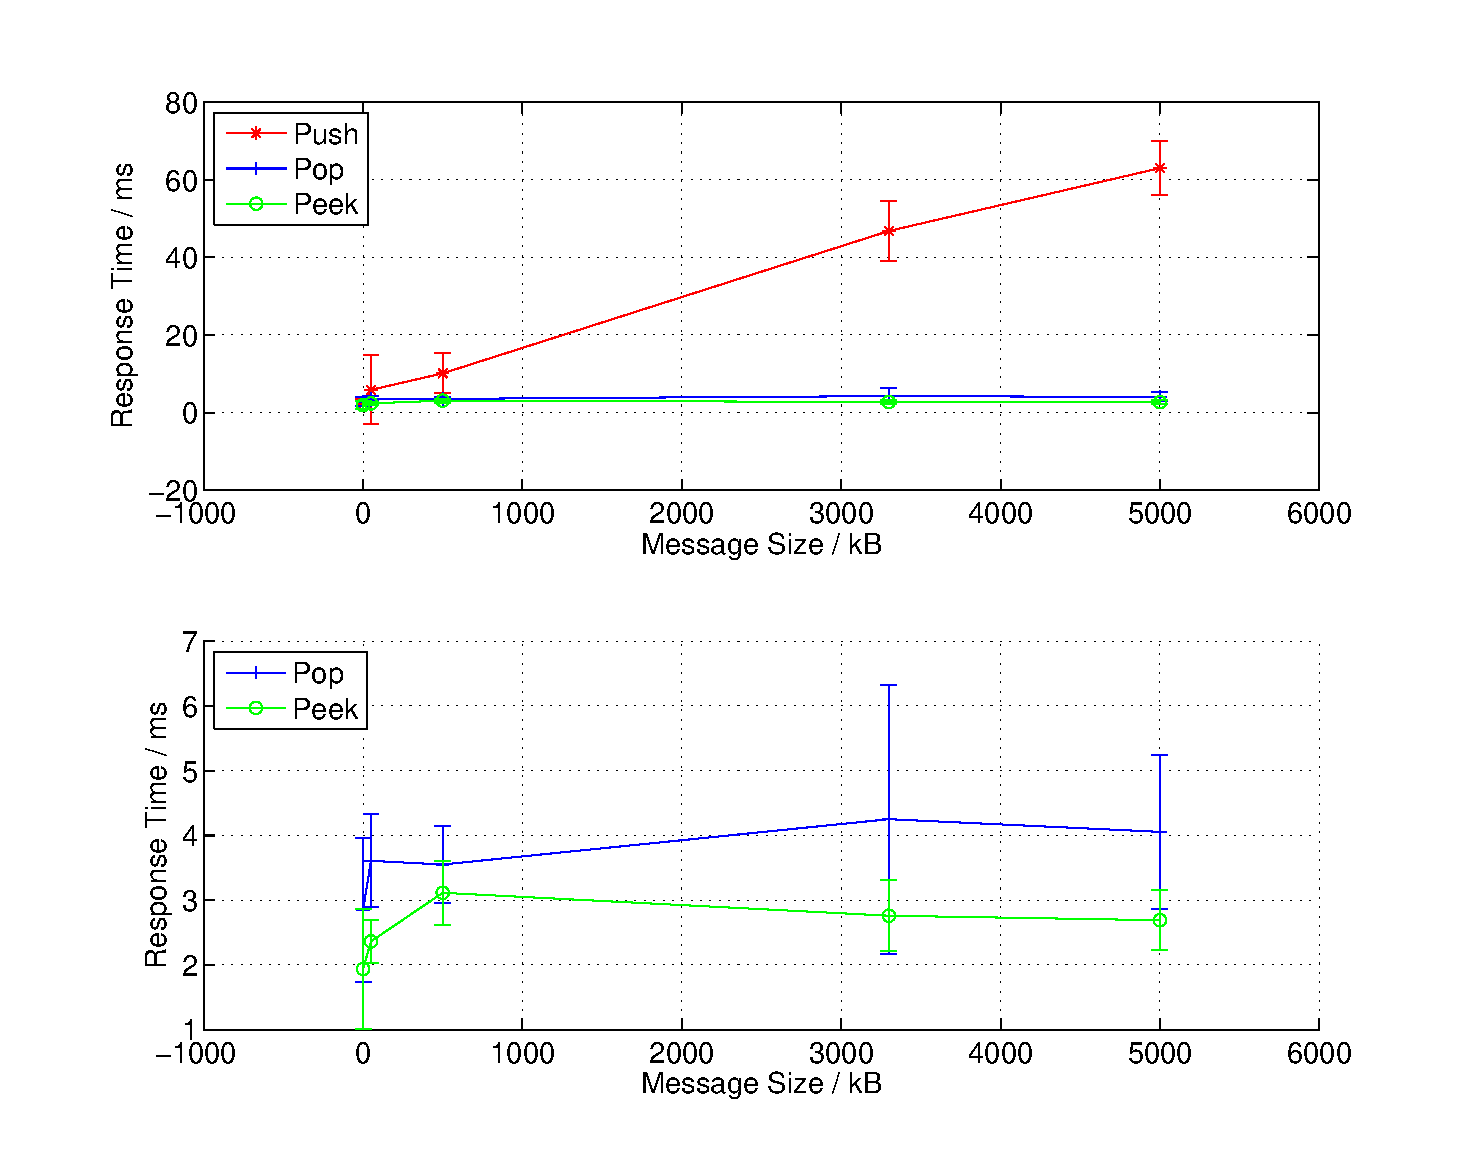
\includegraphics[scale=0.60]{responsetime_msgsize}
                    \caption{The response time for \textit{send message}, \textit{peek message}, and \textit{pop message} as a function of the message size. The peeking and popping curves are also shown again in the lower graph without response time of \textit{send message} for clarity.}
                    \label{fig:responsetime_msgsize}
                \end{figure}
            The raw data from these tests can be found in the log-folder, in the subfolders
            \begin{itemize}
                \item folders
            \end{itemize}

        \subsection{Difference in size of dataset}
            In this test we want to see what the difference of the size of the dataset matters to our system's performance. In this test we're using \textit{Send and Pop Same Client}, varying the number of messages initially stored in the database. From this test we expect that an increase in the size of the data set will increase the think-time of the database, resulting in a lower throughput.
            \begin{figure}[H]
                \hspace{-1.5cm}
                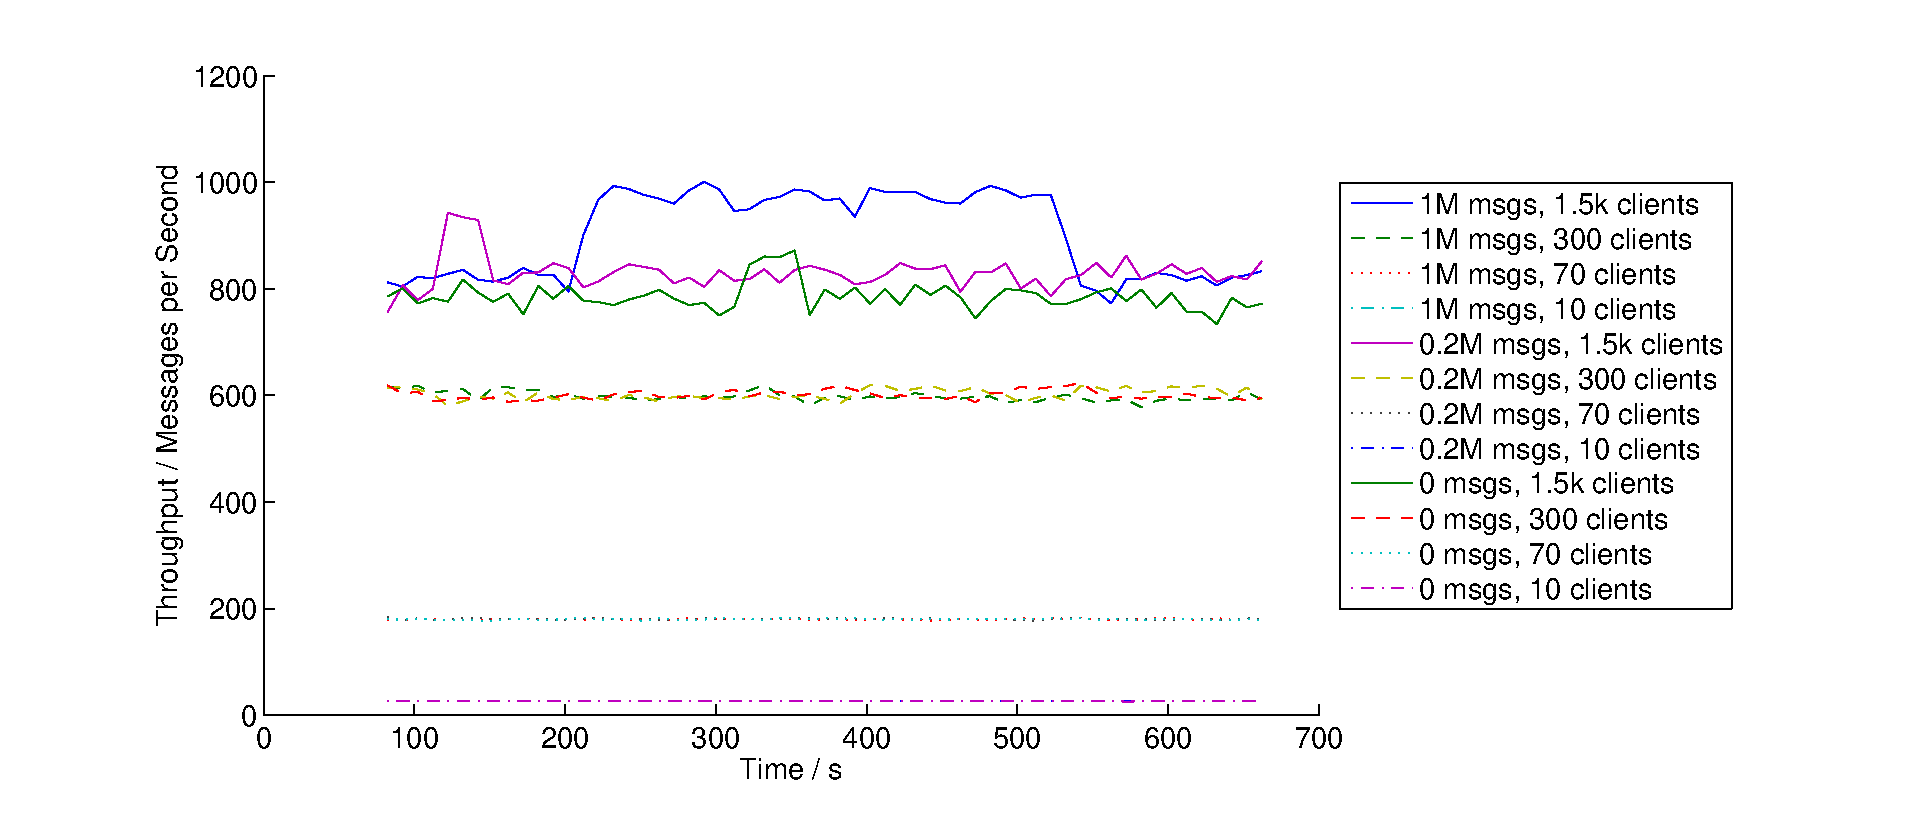
\includegraphics[scale=0.55]{msg_db_clients}
                \caption{The throughput when running \textit{Standard Test} varying number of clients and number of messages stored in database prior to test start. Run on one middleware having 50 worker threads and 50 database connections.}
                \label{fig:msg_db_clients}
            \end{figure}
            ~\\
            \\
            The raw data from these tests can be found in the log-folder, in the subfolders
            \begin{itemize}
                \item \textit{sendandpopsameclient\_diff\_clients\_msgsize-10b}
                \item \textit{sendandpopsameclient\_diff\_clients\_msgsize-1mb}
                \item \textit{sendandpopsameclient\_diff\_clients\_msgsize-10mb}
            \end{itemize}

        \subsection{Difference in number of clients}
            On Figure \ref{fig:msg_db_clients}, looking at tests with the same initial size of the dataset, we see that an increase in clients gives an increase in throughput in all of the tests. 

        \subsection{Difference in frequency of requests}
            \label{sec:difference_in_frequency_of_requests}
            In this test we want to measure the impact on the server when we differ the frequency of requests. We performed 6 \textit{Send and Pop Same Client}-tests, differing only the wait time between requests. The tests were performed using one middleware with 30 database connections and 30 worker threads, and 100 client threads on the client machine.\\
            \\
            In this test we expect to see that the throughput increases with the number of requests, possibly reaching a point where it starts becoming unstable.\\
            \\
            On the left of Figure \ref{fig:sleep_time_between_requests_100clients_30_30} we see that the throughput increases as the wait time decreases, which is another way of saying that the throughput increases when the frequency of requests increases. We also see that the standard deviation increases slightly as the throughput decreases\\
            \\
            In the top right corner of the graph we see that the average time requests spend queuing (waiting to get handed to a worker thread) is higher when the wait time between requests is zero.\\
            \\
            In the lower right corner we see that the combined time spent in Client Request Worker and IPersistence is going up when the frequency of requests increases.

             \begin{figure}[H]
                \begin{adjustwidth}{-2.5cm}{}
                    \centering
                    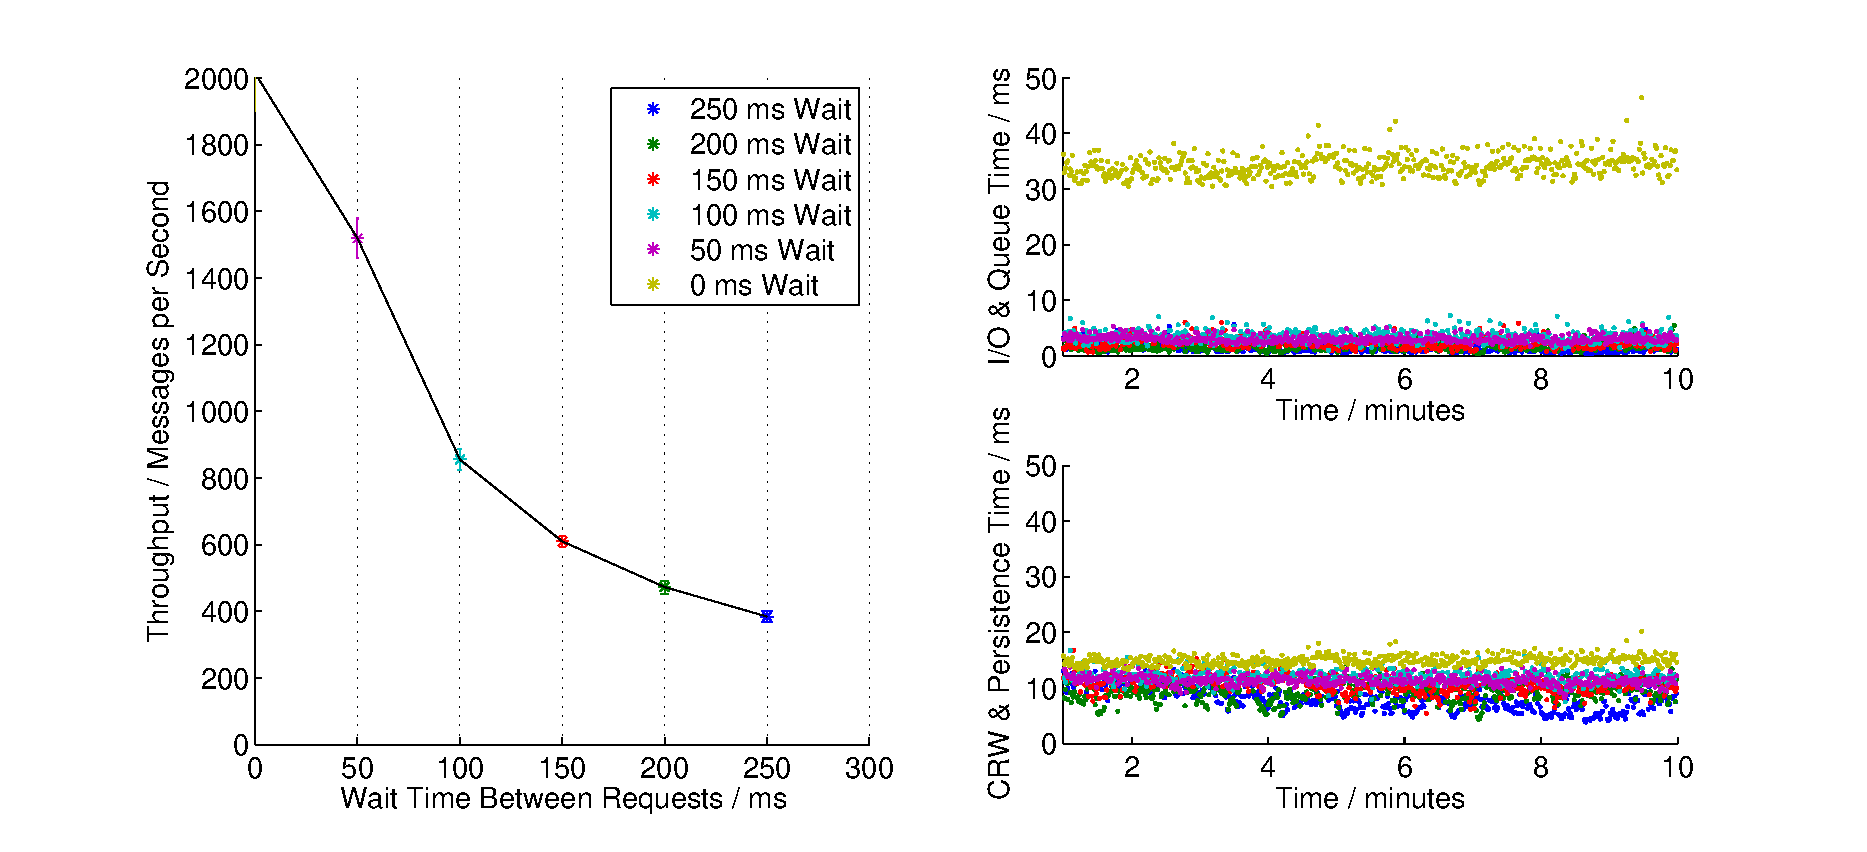
\includegraphics[scale=0.65]{sleep_time_between_requests_100clients_30_30}
                    \caption{\textit{Send and Pop Same Client} test differing the amount of wait time between requests. On the left side we have plotted the throughput when increasing the wait time. In the top right corner we have plotted the average time of Socket IO \& Queue. In the lower right corner we have plotted the sum of \textit{IPersistence} and \textit{Client request worker}}
                    \label{fig:sleep_time_between_requests_100clients_30_30}
                \end{adjustwidth}
             \end{figure}
             ~\\
             \\
             On figure \ref{fig:sleep_time_between_requests_respTime_100clients_30_30} we see that the average response time goes up when we increase the frequency of requests. We also see that the standard deviation of response time increases when the frequency of requests increases.\\
             \\
              \begin{figure}[H]
                \begin{adjustwidth}{-2.5cm}{}
                      \centering
                      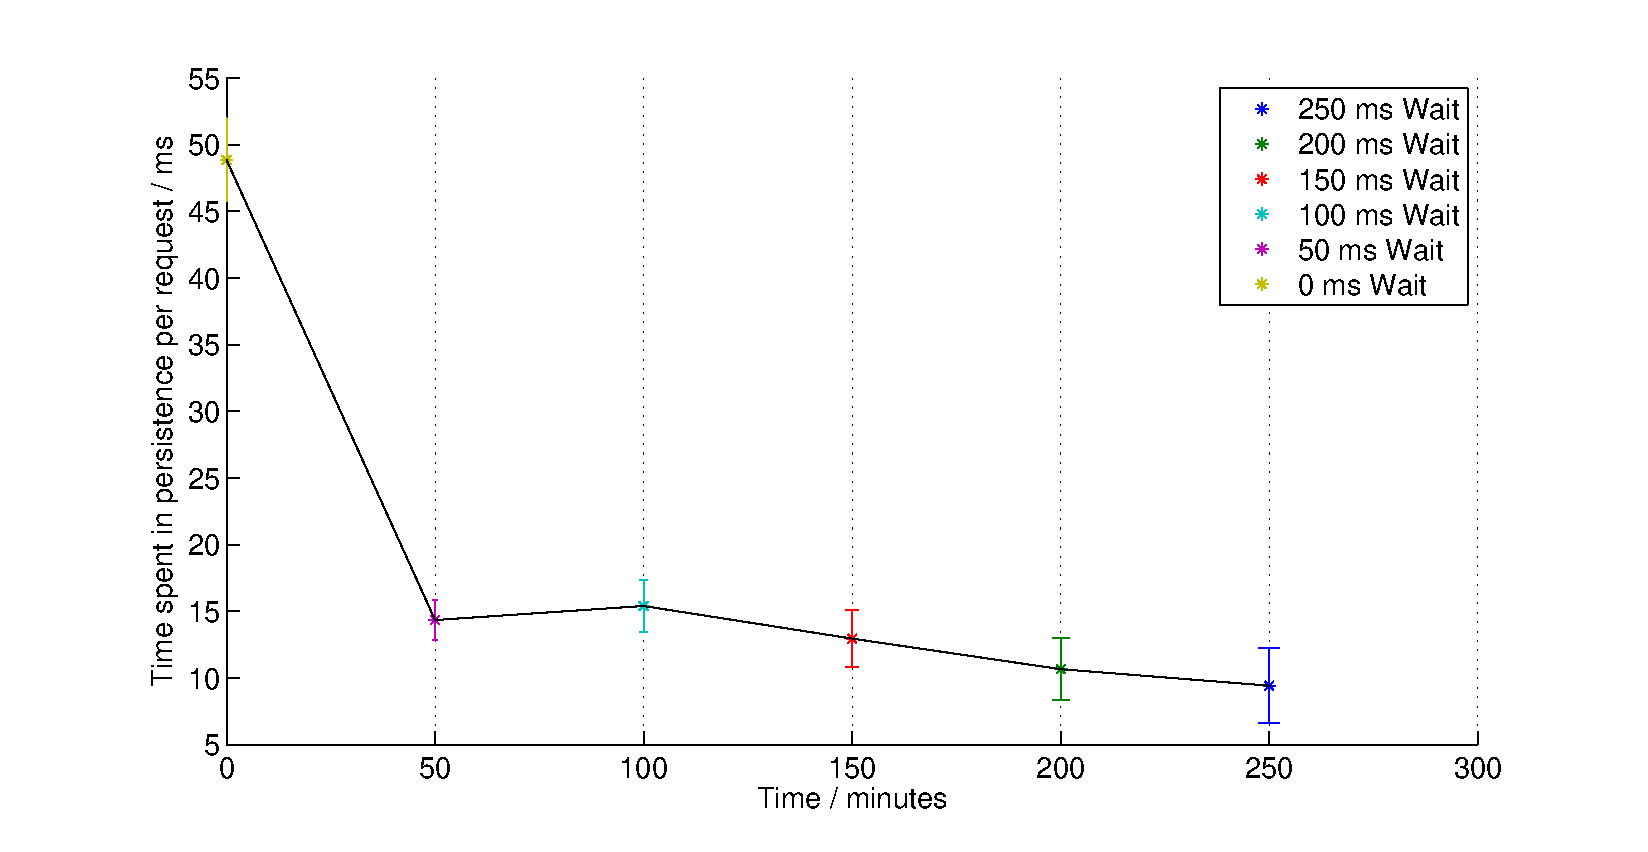
\includegraphics[scale=0.60]{sleep_time_between_requests_respTime_100clients_30_30}
                      \caption{Same test as Figure \ref{fig:sleep_time_between_requests_100clients_30_30}, this time plotting total response time when increasing wait time}
                      \label{fig:sleep_time_between_requests_respTime_100clients_30_30}
                \end{adjustwidth}
              \end{figure}


        \subsection{Difference in data store}
            In this test we measure the difference between using Postgres and not storing anything at all. We expect to see an an increase in throughput since we don't have to communicate with the database at all and thus don't have to wait for the network or database think time.
            
        \subsection{Difference in number of middlewares}
            \begin{figure}[H]
                \hspace{-1.5cm}
                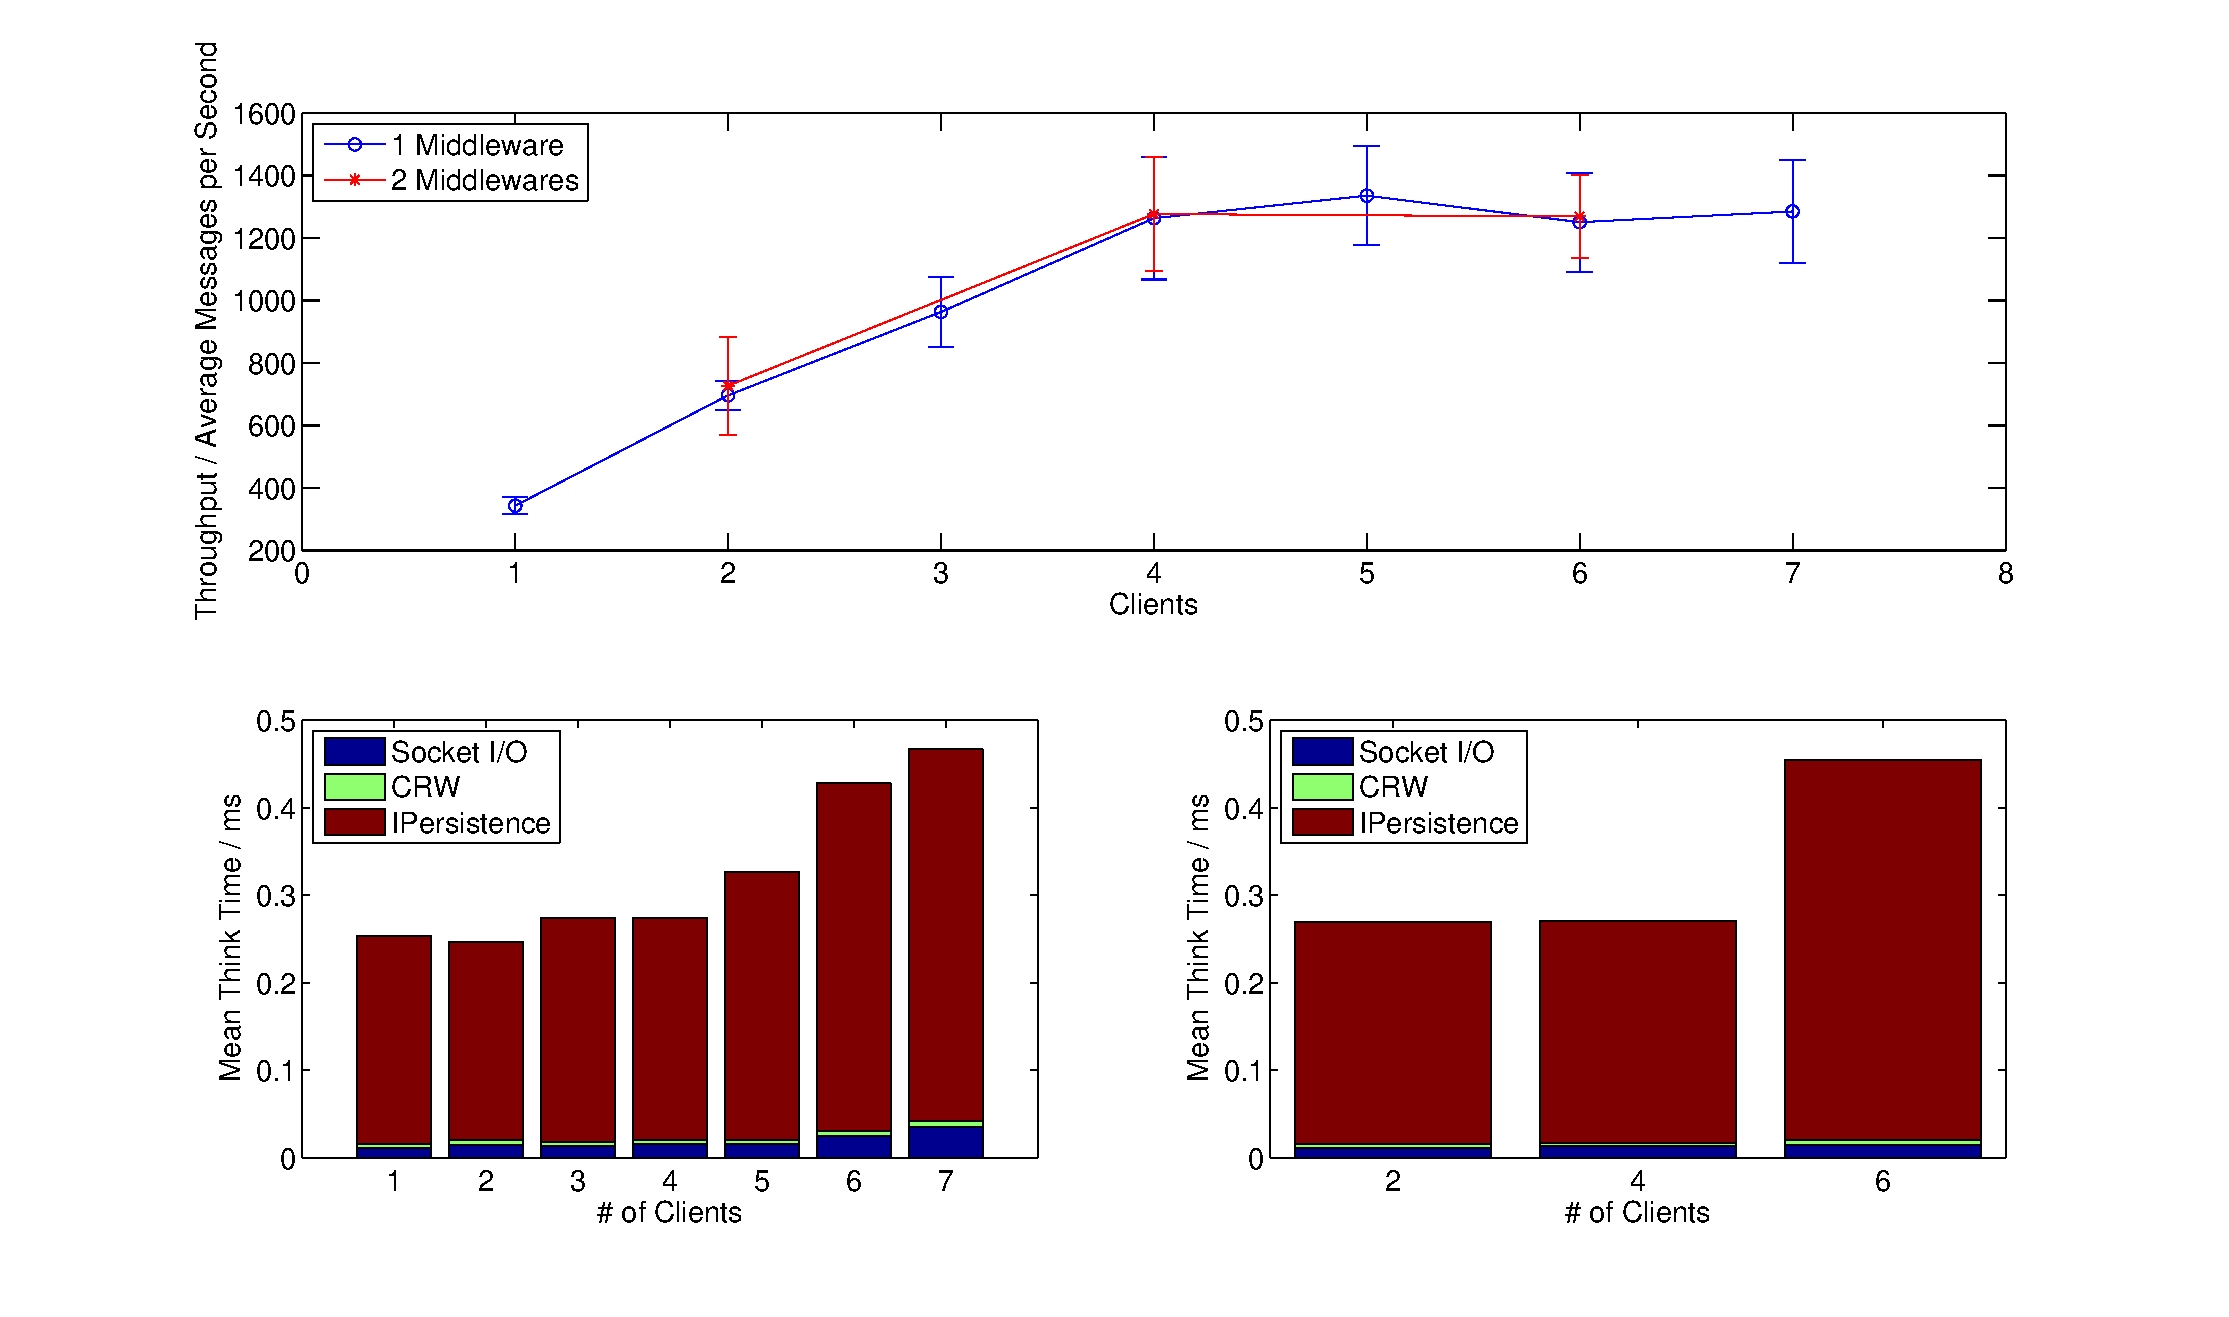
\includegraphics[scale=0.40]{throughout-thinktime_middleware_clients}
                \caption{The throughput when running \textit{SendAndPopSameClient} varying number of clients and number of middlewares.}
                \label{fig:throughput_middleware_clients}
                \end{figure}
            \begin{table}
            
            \begin{tabular}{|c|c|c|c|}
            \hline
            \textbf{1 Middleware} & & &\\
            \hline
            Clients & Socket I/O \& Queuing & Client Request Worker & IPersistence \\ \hline
            1&  111.77 &    48.33 &  2380.06\\ \hline  
 2& 139.26 &    62.93 &  2266.02\\ \hline  
 3& 138.36 &    45.89 &  2553.87\\ \hline  
 4& 153.40 &    47.68 &  2541.67\\ \hline  
 5& 152.72 &    47.07 &  3062.58\\ \hline  
 6& 244.52 &    60.62 &  3974.65\\ \hline  
 7& 345.78 &    76.72 &  4247.42\\ \hline    
            \textbf{2 Middlewares} & & & \\  
                \hline
                Clients &   Socket I/O \& Queuing & Client Request Worker & IPersistence \\ \hline
                 2& 106.68 &    47.79 &  2540.22\\ \hline  
                 4& 129.81 &    36.00 &  2537.58\\ \hline  
                 6& 147.75 &    49.79 &  4351.00\\ \hline  
                \end{tabular}
                \caption{Average think time for middleware components when varying number of clients for 1 and 2 middlewares.}
                \label{table:thinktime_middleware_clients}
            \end{table}                
            
            \begin{table}
                \begin{tabular}{|c|c|c|c|}
                    \hline
                    \textbf{1 Middleware} & & &\\
                    \hline
                    Clients & Socket I/O \& Queuing & Client Request Worker & IPersistence \\ \hline
                    1&   15.62 &     6.49 &   158.56 \\ \hline  
                    2&   28.52 &    11.77 &   147.64 \\ \hline  
                    3&   32.15 &    11.71 &   362.91 \\ \hline  
                    4&     41.51 &    13.32 &   487.37 \\ \hline  
                    5&   24.99 &     9.88 &   441.94 \\ \hline  
                    6&   48.75 &    23.97 &   485.21 \\ \hline  
                    7&   61.23 &    24.84 &   587.43 \\ \hline      
                    \textbf{2 Middlewares} & & & \\  
                        \hline
                        Clients &   Socket I/O \& Queuing & Client Request Worker & IPersistence \\ \hline
                    2&  29.02 &    12.97 &   549.87 \\ \hline  
                    4&  37.73 &    10.67 &   428.83 \\ \hline  
                    6&  35.89 &    10.64 &   708.21 \\ \hline 
                \end{tabular}
                \caption{Think time standard deviation for middleware components when varying number of clients for 1 and 2 middlewares.}
                \label{table:thinktime_std_middleware_clients}
            \end{table}            
            
        \subsubsection{Response Times for Requests}
                \begin{table}
                    \begin{tabular}{|c|c|}
                        \hline 
                        \textbf{Type of Request} & \textbf{Response Time} (ms) \\ 
                        \hline 
                        Pop & $3.997 \pm 0.021$ \\ 
                        \hline 
                        Peek & $2.022 \pm 0.038$ \\ 
                        \hline 
                        Push & $1.856 \pm 0.61294$ \\ 
                        \hline 
                    \end{tabular} 
                    \caption{The response times for the requests: pop push and peek. Using 50 worker threads, 50 db connections, 1 client and 1 middleware.}
                    \label{tbl:response_times_requests}
                \end{table}
		\subsection{$2^2$ Tests}
    		\subsubsection{Worker-threads vs Clients}
    		\begin{table}
    			\begin{tabular}{|c|c|c|}
        			\hline 
        			• & 500/250 & 100/50 \\ 
        			\hline 
        			100/100 & $309.29 \pm 47.7$ & $350.94 \pm 0.68$ \\ 
        			\hline 
        			30/30 & $405.10 \pm 72.90$ & $793.39 \pm 1.32$ \\ 
        			\hline 
			    \end{tabular} 
                \caption{$2^2$ testing for throughput, varying number of client and numer of threads. Test used: Standard test}
                \label{table:2k2-threads-clients}
            \end{table}

        \subsection{Difference in database connections and worker threads}
            \label{sec:difference_in_dbcons_and_worker_threads}
            In this test we perform 3 \textit{Send and Pop Same Client}-tests, differing the amount of worker threads and database connections. As explained in Section \ref{sec:description_middleware} we expect that the throughput of the middleware is bounded by the minimum of the number of worker threads and the number database connections.

             \begin{figure}[H]
                 \centering
                 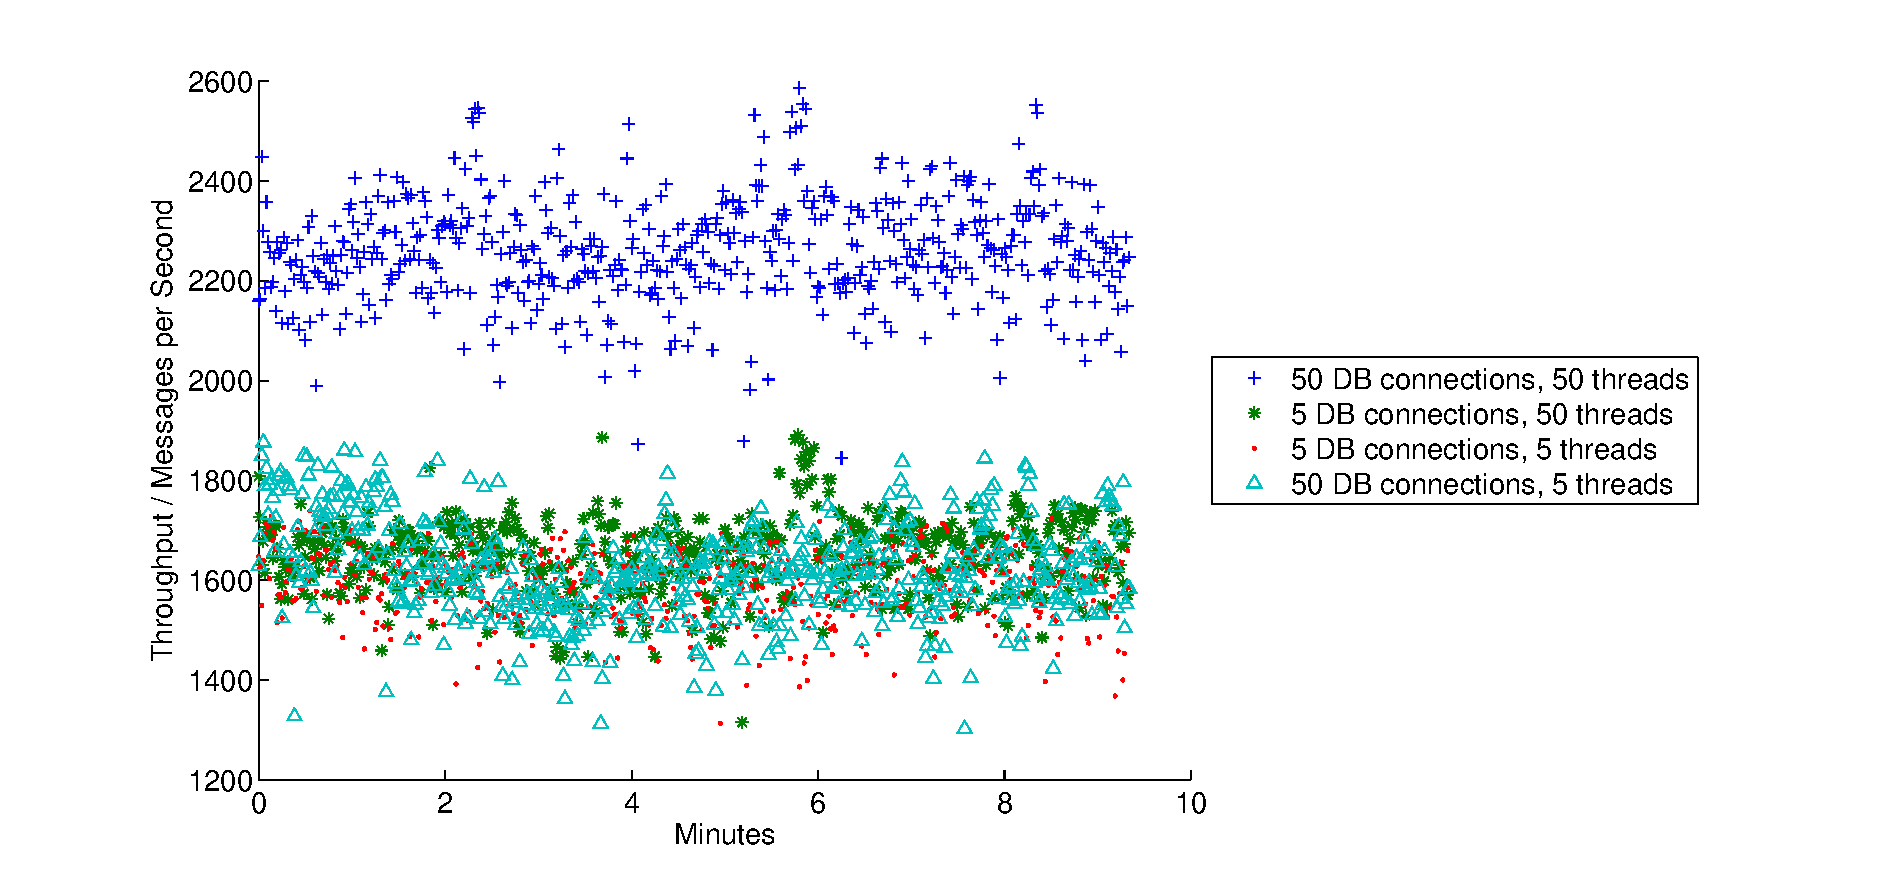
\includegraphics[scale=0.50]{throughput_vs_dbconns}
                 \caption{The combined throughput of \textit{Send Message}- and \textit{Pop message} requests of the system while performing \textit{Send and Pop Same Client}, differing the number of database connections and worker threads on the middleware, performed on a single middleware.}
                 \label{fig:throughput_vs_dbconns}
             \end{figure}
             ~\\
             On Figure \ref{fig:throughput_vs_dbconns} we see that the result seems to be matching our expectations; the throughput is higher when both the number of database connections and worker threads is 50, but stays lower when either the number of database connections or worker threads is 5. Also we notice that the standard deviation of our results seem to increase as the maximum of the number of database connections and worker threads increases.
            % TODO: plot graphs for diff_worker-threads_client-threads-10db-cons-10ms-sleep and diff_worker-threads_client-threads-same-as-db-cons-10ms-sleep
            The raw data from these tests can be found in the log-folder, in the subfolders
            \begin{itemize}
                \item folders
            \end{itemize}
            
    \section{Analysis}
        \label{sec:analysis}
        In this section we interpret and compare the results shown in \ref{sec:tests_and_results} above, in order to figure out what the different performance metrics of our system are.

        \subsection{Time spent in each part of the system}
            \label{sec:time_spent_in_each_part_of_the_system}
            % TODO USE DATA FROM diff_db-cons_worker-threads_i-fooled-you VS diff_num-db-threads AS WELL
            In order to determine how much time is spent in each part of our system, we look at the results we measured during code profiling (Figure \ref{fig:code_profiling_send_pop_same_client} and \ref{fig:code_profiling_standard_test}) and the data we have on the bottom of Figure \ref{fig:throughput_middleware_clients}.\\
            \\
            The results of our code profiling show that 83-87\% of our codes' execution time is spent waiting for replies from the database. It is important to note that this time \textbf{includes} the network delay between the middleware and the database, in both directions.\\
            The results from the code profiling are backed up with our own logging data, where we have also measured how much time is spent in different parts of our system. On Figure \ref{fig:throughput_middleware_clients} we also have evidence that the server spends most of its time waiting for a response from the database, waiting in the IPersistence class of our implementation.\\
            \\
            This data all points to the database or the network being the bottleneck in these particular tests. We contribute this to choosing bad indexes for our data, having a poorly configured database, or having a slow network.

            % USE:
            %   1) diff_db-cons_worker-threads_i-fooled-you VS diff_num-db-threads
            %   2) Code profiling above
            %   3) Plots showing CRW, IO, and DB
            % SHOW:
            %   1 -> we have WAY better performance with i_fooled_you
            %   2 -> our profiling shows that we spend WAY more time doing db-stuff than anything else
            %   3 -> our measurements show that we wait a lot for the database, compared to anything else
            % CONCLUDE:
            %   We spend a lot of time in the database, which might be because of bad configuration, indexes etc.

        \subsection{Size of messages}
            % USE: 
            %   1) diff_clients_msgsize-10b VS diff_clients_msgsize-1mb VS diff_clients_msgsize-10mb
            %   2) fig:responsetime_msgsize
            % SHOW:
            %   1 -> it doesn't seem to matter much
            %   2 -> it seems to matter for push
            % CONCLUDE:
            %   THIS MIGHT BE A BIT TOO CONTRIVED:
            %   We have one component that performs so poorly that our other configurations don't really seem to matter

        \subsection{Number of middlewares}
            % USE
            %   1) fig:throughput_middleware_clients
            %   2) response time data from test in 1)
            % SHOW:
            %   1 & 2 -> throughput increases with the number of clients
            %   1 & 2 -> response time decreases with the number of middleware. This is because of #worker-threads which limits the amount of simultaneous requests.

        \subsection{Number of clients}
            % USE
            %   1) 2H tests
            %   2) 
            % SHOW:
            %   1 -> throughput goes up as number of clients increases


        \subsection{Stability of the system}
            In our long trace tests we saw that our system behaved in a reasonably stable manner over both two and four hour tests.

            150 clients: This data shows that we are not yet pushing the system to the point of making it unstable, low standard deviation\\
            \\
            750 clients 100 dbcons: At this point we see a significant increase in the standard deviation. We note that the throughput is much higher, which is caused by the increased amount of requests. Here we could reference \ref{sec:frequency_of_requests}, saying that there are always requests in the queue, and we don't have any wait time.\\
            \\
            Increased throughput when decreasing num-dbcons and wthreads, but increased number of clients. The reason is queuing in the middleware.

        \subsection{Frequency of requests}
            \label{sec:frequency_of_requests}
            % USE
            %   'Difference in number of clients'
            %   'Differency in frequency of requests'
            % SHOW
            %   We've shown that the system didn't reach its' limit yet, but the big deviation we get with many requests (many clients) shows that we might reach that point
            As noted in Section \ref{sec:difference_in_frequency_of_requests} we see on Figure \ref{fig:sleep_time_between_requests_100clients_30_30} that the throughput of our system goes up when the frequency of requests increases. This seems reasonable, and points to the fact that our system can handle more load than the test produces when the wait time is relatively high. What seemed to be counter-intuitive to us in the beginning was that the average response time (as shown on Figure \ref{fig:sleep_time_between_requests_respTime_100clients_30_30}) is much higher when the wait time is lower, even though the throughput is much higher at the same time! After plotting the top right part of Figure \ref{fig:sleep_time_between_requests_100clients_30_30}, we realized that this must be because there are many requests queued, waiting to be served. This gives a higher throughput since the server always has a new request to process and at the same time gives a higher average response time since there are requests waiting to be served in the queue.\\
            \\
            As we also noted in Section \ref{sec:difference_in_frequency_of_requests} the standard deviation of response time becomes higher as the average response becomes lower, and the frequency of messages decreases. What's happening at this point is that the requests are so infrequent that there is (almost) no queuing in the middleware, causing requests to be processed immediately. When the average response time becomes as low as 10 milliseconds, it is seems very reasonable to us that the standard deviation increases, since things such as network i/o will play a big part in the result.\\
            \\
            Finally we note that our system seems to be performing best (in this particular setup) when the wait time between requests is around 50-60 milliseconds, an average of 1500-1600 requests per second (when the distribution of requests is half \textit{Pop message} and half \textit{Send message}), since this is the point where the throughput is relatively high while the average response time hasn't begun increasing drastically yet.

        \subsection{Bound on throughput of middleware}
            \label{sec:analysis_bound_on_throughput}
            On Figure \ref{fig:throughput_vs_dbconns} we saw that, as per our expectations, the throughput of the middleware (assuming a high enough frequency of requests) is bounded by the minimum of the number of database connections and the number of worker threads. This is a very intuitive result since each worker thread will use exactly one database connection per (well formed) request. This means that if we want to keep the utilization of both worker threads and database connections high, we should keep the ratio between them 1, as other ratios would leave one of the resources idle.\\
            This result is backed up by the results of our long traces where, in Table \ref{table:long_trace_test_summary_sendmessage} and \ref{table:long_trace_test_summary_popmessage}, we saw that increasing the amount of database connections and worker threads also resulted in a higher standard deviation in throughput.\\
            \\
            In both of the mentioned tests we also see that the standard deviation of the results seems to be increasing when the amount of worker threads and database connections is increased. We attribute this to the fact that we give the database more work to do simultaneously, causing a higher response time for the database.\\
            \\
            If we look at the measured think-time of the database during the long traces, we see that this confirms our suspicion; the think-time of the database increases when we increase the amount of worker threads and database threads.

        \subsection{Micro benchmarks}
            \label{sec:analysis_micro_benchmarks}
            TODO: Pop message: It seems that some external factor might be causing this, for instance we have Postgres' automatic VACUUM activated. It could be that the trend we see decreases with time because the number of messages in the database decrease and that the VACUUM operation therefore takes less time

    \section{Conclusion}
        % More middleware does not increase throughput because the database is the bottle neck, and is shared among all middleware.
        % Increasing # middleware can give a lower response time, if there are enough requests (vs worker threads and db cons) to form queues in the middleware

        In Section \ref{sec:difference_in_dbcons_and_worker_threads} we found that the performance of our middleware depends, among other things, on the ratio between the amount of worker threads and database connections. In this section we found that the ratio should be 1 if we want to utilize all of our database connections and worker threads simultaneously. This was a very intuitive result to us, and was exactly what we expected to see.\\
        \\
        Not only does the ratio between worker threads and database connections matter, so does the \textit{number} of worker threads and database connections.\\
        \\
        In our analysis in Section \ref{sec:time_spent_in_each_part_of_the_system} we found that found that during execution of our middleware, most of the time is spent waiting in the IPersistence class or, more specifically, waiting for responses from the database. This result is consistent with the test results from the other tests we made that put a significant load on the system. This implies that, in our current setup, the database is the bottleneck. We do not blame this on the database implementation, but rather on ourselves, for choosing bad indexes and/or configuring the database poorly w.r.t. the dataset and the type of queries our system has and performs.\\
        If we had had more time to test our system we would try to change the indexes and rerun our tests to see how much performance we could gain from a more appropriate configuration of the database.
        % TODO: It's better to have more worker threads, but only up to a certain point. We have data that shows that it's better to have 30 worker threads than 100 in some situations
    \clearpage
    \appendix
        \section{Message protocol and API}
        \label{sec:message_protocol_api}
            \subsection{Exceptions}
                If a request cannot be fulfilled by the server, the server will respond with an exception.  Exceptions have the following format:\\
                \\
                \indent\textit{FAIL $<$type$>$ $<$id$>$}\\
                \\
                Where $<$type$>$ is either QUEUE, CLIENT, MESSAGE, or UNKNOWN, and where $<$id$>$ is the id of the queue, client or message that ‘failed’. For instance, if a client tries to send a message to the queue with id 5 and if that queue doesn’t exist, the server will respond with “FAIL QUEUE 5”.

            \subsection{Handshake}
                The client should send HELLO when first connecting to the server. The server should respond with OK if it accepts the client, otherwise the server should respond with something else. The client must disconnect if it receives anything other than OK from the server.


            \subsection{Send Message}
                \indent\indent\textit{MSG,ReceiverId,SenderId,QueueId,Priority,Context,Content}\\
                \\
                \textbf{Response}\\
                The server should respond with OK if the message was inserted into the queue successfully, otherwise it should respond with FAIL.\\
                \\
                \textbf{Remarks}\\
                To send a message to multiple queues, separate the QueueIds with a semicolon, e.g. 1;2;3 to send the message to queues 1, 2 and 3.

            \subsection{Message Response}
                \indent\indent\textit{MSG,SenderId,Context,MessageId,Content}\\
                \\
                This is here to save space in the definitions below. This is how the server should return a message upon request from the client.

            \subsection{Peek Queue}
                \indent\indent \textit{PEEKQ,ReceiverId,QueueId,OrderByTimestampInsteadPriority}\\
                \\
                \textbf{Response}\\
                The server should respond with the message formatted as in section 1.2 if there is a message in the queue. Otherwise the response should be MSG0.\\
                \textbf{Remarks}\\
                OrderByTimestampInsteadPriority is either 1 or 0.

            \subsection{Peek Queue with Specific Sender}
                \indent\indent\textit{PEEKS,ReceiverId,QueueId,SenderId,OrderByTimestampInsteadPriority}\\
            \\
            \textbf{Response}\\
            The server should respond with the message formatted as in section 1.2 if there is a message in the queue. Otherwise the response should be MSG0.\\
            \\
            \textbf{Remarks}\\
            OrderByTimestampInsteadPriority is either 1 or 0.


            \subsection{Pop Queue}
                \indent\indent\textit{POPQ,ReceiverId,QueueId,OrderByTimestampInsteadPriority}\\
                \\
                \textbf{Response}\\
                The server should respond with the message formatted as in section 1.2 if there is a message in the queue. Otherwise the response should be MSG0.\\
                \\
                \textbf{Remarks}\\
                OrderByTimestampInsteadPriority is either 1 or 0.

            \subsection{Pop Queue with Specific Sender}
                \indent\indent\textit{POPS,ReceiverId,QueueId,SenderId,OrderByTimestampInsteadPriority}\\
                \\
                \textbf{Response}\\
                The server should respond with the message formatted as in section 1.2 if there is a message in the queue. Otherwise the response should be MSG0.\\
                \\
                \textbf{Remarks}\\
                OrderByTimestampInsteadPriority is either 1 or 0.

            \subsection{Create Queue}
                \indent\indent\textit{CREATEQUEUE,NameOfQueue}\\
                \\
                \textbf{Response}\\
                The server should respond with the id (long) of the queue, if a queue with the same name exists the server should respond with FAIL.

            \subsection{Remove Queue}
                \indent\indent\textit{REMOVEQUEUE,QueueId}\\
                \\
                \textbf{Response}\\
                The server should respond with OK or FAIL.

\end{document}
